% -----------------------------------------------------------------------------
% Paquetes y configuracion
% -----------------------------------------------------------------------------
\documentclass[11pt,twoside]{report}
% \usepackage{fancyhdr}
\usepackage[a4paper,width=170mm,top=25mm,bottom=25mm,bindingoffset=6mm]{geometry}
\usepackage[acronym]{glossaries}
\usepackage[backend=biber]{biblatex}  % bibliografia
\usepackage[spanish]{babel}
\usepackage[utf8]{inputenc}
\usepackage{amsmath}
\usepackage{amssymb}
\usepackage{booktabs}
\usepackage{csquotes}
\usepackage{graphicx}
\usepackage{longtable}
\usepackage{rotating}

% Abreviaciones
\newacronym{ag}{AG}{Algoritmo genético}
\newacronym{mrcvc}{MRCVC}{Motor rotativo de combustión a volumen constante}
\newacronym{rans}{RANS}{\emph{Reynolds-average Navier-Stokes}}
\newacronym{dta}{DTA}{Diámetro del tubo de admisión}
\newacronym{dte}{DTE}{Diámetro del tubo de escape}
\newacronym{lta}{LTA}{Longitud del tubo de admisión}
\newacronym{lte}{LTE}{Longitud del tubo de escape}
\newacronym{iia}{IIA}{Ángulo de apertura del puerto de admisión}
\newacronym{ifa}{IFA}{Ángulo de cierre del puerto de admisión}
\newacronym{eia}{EIA}{Ángulo de apertura del puerto de escape}
\newacronym{efa}{EFA}{Ángulo de cierre del puerto de escape}
\newacronym{unl}{UNL}{Universidad Nacional del Litoral}
\newacronym{unco}{UNCo}{Universidad Nacional del Comahue}

% Nomenclatura
\newglossaryentry{reynolds}{
    name = $R_e$ ,
    description = Número de Reynolds
}
\newglossaryentry{rend_vol}{
    name = $\eta_v$ ,
    description = Rendimiento volumétrico
}
\newglossaryentry{dens_atmo}{
    name = $\rho_{a,i$ },
    description = Densidad del aire atmosférico
    }
\newglossaryentry{vel}{
    name = $V$ ,
    description = Velocidad
}
\newglossaryentry{ang_ciclo}{
    name = $\theta_c$ ,
    description = Ángulo de ciclo
}
\newglossaryentry{ang_cig}{
    name = $\theta_g$ ,
    description = Ángulo del cigüeñal
}

  % esto esta mejor si lo pongo en cada entrada de texto

\makeglossaries

\addto\captionsspanish{%
    \def\tablename{Tabla}%
}

\graphicspath{ {figuras/} }
\addbibresource{bib.bib}

\pagenumbering{roman}

% \fancyhead{}
% \fancyhead[RO,LE]{Proyecto Integrador Profesional}
% \fancyfoot{}
% \fancyfoot[LE,RO]{\thepage}
% \fancyfoot[LO,CE]{Capítulo \thechapter}
% \fancyfoot[CO,RE]{Nicolás Daniel Barrios}

% -----------------------------------------------------------------------------
% Documento
% -----------------------------------------------------------------------------
\begin{document}

% -- Iniciales
\begin{titlepage}
    \begin{center}

        \vspace*{2cm}
        \huge
        \MakeUppercase{\textbf{Diseño de los sistemas de admisión y escape del
        Motor Rotativo de Combustión a Volumen Constante }}

        \vspace{0.8cm}
        Nicolás Daniel Barrios
        \vfill

        \vspace{0.8cm}
        
\includegraphics[width=0.5\textwidth]{logo_unco.jpg}
        \vspace{0.8cm}


        \large
        Facultad de Ingeniería \\
        Universidad Nacional del Comahue \\
        Argentina \\
        2021
    \end{center}
\end{titlepage}

\setcounter{page}{1}
\section*{Agradecimientos}
A mi familia y amigos.

\section*{Resumen}
Aca un pequeño resumen.

\tableofcontents
\listoffigures
\listoftables
\printglossary[type=\acronymtype,title=Abreviaciones]
\printglossary[title=Nomenclatura]

% -- Cuerpo del texto
\pagenumbering{arabic}
\chapter{Introducción}

Este trabajo presenta un procedimiento para optimizar la geometría del sistema
de intercambio de gases del \gls{mrcvc}
\cite{toth}, en particular de la geometría y posición en el cuerpo estatórico
de los puertos de admisón y escape, diámetro y longitud de los conductos
corresponidentes.

El MRCVC es un proyecto nacido en la Universidad Nacional del Comahue en el
marco del \emph{Proyecto de Investigación Desarrollo de modelos y herramientas
para la simulación de problemas complejos en ingeniería mediante
fluidodinámica computacional (04/I-251)}. Actualmente se encuentra en etapa
de desarrollo.

La optimización de la geometría se realizó con un conjunto de herramientas, en
primer lugar para obtener las curvas de redimiento volumétrico se utilizó un
simulador de motores de combustión interna, 

Se utilizó un simulador de motores de combustión interna para simular obtener
las curvas características del motor, curvas que se utilizan para dar un
puntaje a una algoritmo genético para optimizar el conjunto de parámetros que
definen la geometría de los sistemas de intercambio de gases y 

La motivación de este trabajo surge de continuar con el desarrollo del Motor
Rotativo de Combustión a Volumen Constante (MRCVC), en particular
mejorar el prediseño de los sistemas de intercambio de gases sentando las bases
para una futura optimización de los mismos en un motor con requisitos de diseño
establecidos.

\chapter{Antecedentes} \label{cap:antecedentes}

\section{Motor Rotativo de Combustión a Volumen Constante}
%
El MRCVC es un proyecto que surgió en la Universidad Nacional del
Comahue, inventado y patentado en el año 2004 por Jorge Toth\cite{toth}.
%
Actualmente se encuetra en desarrollo en el Departamento de Mecánica Aplicada
de la UNCo, en el marco del Proyecto de Investigación Desarrollo de modelos y
herramientas para la simulación de problemas complejos en ingeniería mediante
fluidodinámica computacional (04/I-251).

En trabajos anteriores\cite{lopez16, lopez13, roldan} se han mencionado las
características que hacen al MRCVC un motor atractivo. La geometría de la cámara
de combustión y del conjunto rotante permiten  combustión a volumen constante y
un balanceo mecánico de fuerzas.
%
Esto permite un funcionamiento más suave del motor, además de una reducción del
ruido y desgaste en comparación a motores rotativos tradicionales (Wankel) y
alternativos.


No obstante a esto hay que mencionar que los motores rotativos traen consigo una
serie de problemas como la necesidad de introducir aceite a la cámara de
combustión para lubricar elementos móviles, el solape de cámaras durante la
apertura de los puertos y en particular al MRCVC un complejo sistema de
sellos\cite{roldan}.



\section{Sistema de Intercambio de Gases}
%
Este sistema cumple la función de extraer los gases quemados de la cámara de
combustión de manera eficiente al final de cada carrera de expansión y de
admitir una carga de mezcla fresca para el próximo ciclo.
%
% En un motor de cuatro tiempos, el sistema suele estar compuesto por un filtro
% de aire,  tubo que conecta el filtro con el cuerpo de mariposa, cuerpo de
% mariposa, plenum de admisión y un puerto de admisión, como se ve en la
% figura \ref{fig:sist_intercambio}.
%
La masa de aire inductada imita la cantidad de combustible que se puede quemar,
por este motivo es importante tener un sistema de admisión eficiente.
%
De la misma manera, la cantidad de gases quemados que se pueden extraer luego de
cada ciclo limita la cantidad de masa fresca que puede ingresar a la cámara de
combustión.
%
Otros objetivos del sistema de intercambio de gases son el de preparar la
mezcla\footnote{En el caso de motores SI que admiten mezclas de aire y
combustible} y brindar un flujo que favorezca el proceso de combustión.

% \begin{figure}[h!] \centering
% 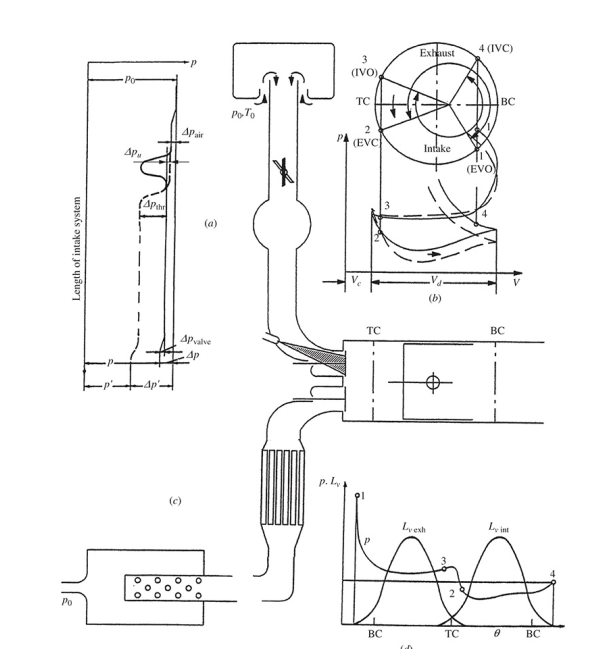
\includegraphics[width=0.5\textwidth]{sistema_intercambio_gases.png}
% \caption{Sistema de intercambio de gases esquematizado(buscar una libre o hacer
% un esquema propio)} \label{fig:sist_intercambio} \end{figure}

Para la simulación del MRCVC se usa una sistema simplificado, que consta de un
tubo de diámetro $D$ y longitud $L$ tanto para la admisión como para el escape,
como se ilustra en la figura \ref{fig:sist_int_mrcvc}.
%
La apertura y cierre de los puertos es controlada por la posición angular de los
puertos en el estator.

% \subsection{Solape de cámaras}
% %
% Es un proceso que ocurre en ambos puertos y que debe ser tenido en cuenta a la
% hora de evaluar el comportamiento del sistema de admisión y escape.
% %

\subsection{Indicadores de rendimiento}

Se medirá la eficiencia del sistema de intercambio de gases utilizando
exclusivamente el rendimiento volumétrico, $\eta_v$.
% Los conductos de admisión restringen el flujo de aire hacia el motor, para
% medir la eficiencia con la que se está admitiendo aire al motor se define el
% rendimiento volumétrico $\eta_v$.
%
Este se define como la relación entre el caudal volumétrico de aire que ingresa
al sistema de admisión y la velocidad a la que cambia el volumen dentro de un
cilindro.


\begin{equation}
  \label{eq:rendVol}
  \eta_v = \frac{2 \dot{m}_a}{\rho_{a,i} V_d N}
\end{equation}

Donde: $\rho_{a,i}$ es la densidad del aire a la entrada del sistema de
admisión (para motores naturalmente aspirados). También se puede definir
$\eta_v$ como:

\begin{equation}
    \label{eq:rendVol2}
    \eta_v = \frac{m_a}{\rho_{a,i} V_d}
\end{equation}

Dónde $m_a$ es la masa inductada al cilindro en cada ciclo.

Hay varios factores que afectan al rendimiento volumétrico, entre los más
importantes están:
%
\begin{enumerate}
    %
    \item Efectos cuasiestáticos
    %
    \item Pérdidas de carga por fricción viscosa
    %
    \item Pérdidas de carga en los puertos de admisión y escape
    %
    \item Transferencia de calor en sistema de admisión
    %
    \item Reglaje de los válvulas/puertos
    %
    \item Bloqueos de flujo en puertos de admisión y escape
    %
    \item Transferencia de calor en el cilindro
    %
    \item Sintonía del puerto de admisión y escape
    %
    \item Métodos de sobrecarga 
\end{enumerate}

Para este trabajo es de interés particular la pérdida de carga en los puertos,
el reglaje y la sintonía de admisión y escape.
%
En \cite{lopez13} se demostró que se tiene una mejor \emph{performance} del
motor si se ubican los puertos en el cuerpo central del estator, realizando un
optimización de la geometría mediante un barrido paramétrico de las variables
geométricas que determinan la forma, posición y reglaje de los puertos.
%
% La ubicación angular de los puertos determina la duración de los procesos de
% admisión y escape, además de modificar la forma y el coeficiente de descarga.

Estos parámetros se ajustan o seleccionan teniendo en cuenta requisitos de
funcionamiento del motor, por lo que fue necesario establecer una curva de
rendimiento volumétrico para que la simulación numérica del
ciclo termodinámico se pueda acoplar al algoritmo de optimización y de este
modo evaluar los motores contra la curva de rendimiento requerida.
%
El criterio de diseño/selección de la curva de $\eta_v$ fué el siguiente:

\begin{itemize}
  \item que tenga un pico de rendimiento entre 4000 y 6000 rpm.
  \item que la curva sea suave
\end{itemize}

% \subsubsection{Fracción de gases residuales}
% %
% A diferencia de un motor alternativo convencional en el que, por medio de
% métodos de sobrecarga se podría reducir la cantidad de gases residuales a una
% fracción despreciable, en el MRCVC, dada la disposición de la geometría siempre
% se transfiere gas residual desde una cámara que está transcurriendo por el
% barrido a la cámara contigua que está iniciando el proceso de admisión.

% Esta masa residual se puede calcular y depende del volumen atrapado y la preisón
% cuando cierra el puerto de escape.
% %
% Esta masa residual marca una cota inferior a la fracción de gases residuales
% que se pueden obtener, se menciona esto porque es un indicador del rendimiento
% de los sistemas de intercabmio de gases.
% %
% Considerando un motor con geometría perfecta y sin pérdida de masa entre los
% sellos, $x_{r\ min}$ se puede calcular como:

% $$
% x_{r\ min} = 0
% $$

% Considerando los valores gemoétricos utilizados para realizar esta optimización,
% este valor de $x_{r\ min}=0.1$ representa un objetivo para este trabajo.

% \subsection{Flujo a través de las válvulas}
% %
% Durante el escape, el soplido es un proceso que puede favorecer a la descarga
% de una cámara.

\subsection{Estrategias de simulación de motores}
%
Se simulará el motor con el simulador de motores de combustión interna ICEsym,
este simulador utiliza modelos 0D para la combustión y 1D para el flujo de
gases a través de los conductos (fuera de la cámara de combustión).

Esta es una herramienta muy útil ya que permite evaluar la \emph{performance} de
un motor a un costo computacional bajo además, la manera en que se implementó la
entrada y salida de datos permite utilizar este simulador como una ``caja
negra'' de modo que se pudo implementar en un \emph{script} como una función a
la que se le otorga como entrada un conjunto de parámetros y devuelve los
resultados de la simulación en un formato que permite la lectura y evaluación de
los mismos.
%
Esta característica del programa la que permitió acoplarlo con un algoritmo
genético para realizar la optimización de la geometría.


Como se mencionó en el apartado \ref{sec:rend_vol}, en trabajos previos se
realizó un pre diseño de los puertos de admisión y escape.
%
En dicho trabajo se determinó coeficientes de descarga constantes
% En dicho trabajo se utilizaron coeficientes de descarga estimados y constantes
para simular el flujo en los puertos de admisión y escape.
%
Con el objetivo de modelar con mayor precisión el flujo a través de los puertos
se realizó una modificación al código de ICESym que permite utilizar una
variable adicional para modelar al $C_d$, con lo que se puede representar la
dependencia con la apertura del puerto como con la diferencia de presión
instantánea como $C_d = f(lv, \delta P)$.

\chapter{MRCVC}

\section{Simulación computacional del ciclo termodinámico MRCVC}

% \section{ICESym}
%
Para simular el ciclo operativo del motor, se utilizó el simulador de motores
de combustión interna ICESym \cite{icesym},
desarrollado en conjunto por la UNCo y UNL.
%
Este simulador utiliza modelos unidimensionales para simular el flujo en los
conductos de admisión y escape y modelos cero dimensionales para el resto de
los componentes.
%
Incluye un modelo para el solape entre cámaras \cite{lopez16} y modificaciones
particulares al MRCVC, para este trabajo en particular  y con el fin de obtener
una mapa del coeficiente de descarga, se ha agregando la diferencia de presión
entre cámara y puerto como variable de modo que $Cd = f(L_v, \delta P)$.

\subsection{Ciclo operativo}
% La combustión se realiza a volumen constante, por lo que es de esperarse
% mayores rendimientos de conversión de combustible en relación a motores en los
% que la combustión no se realiza a volumen constante.

% hace falta mostrar que esto es así? poner algún gráfico del heywood o cosas
% por el estilo. puedo citar el heywood?

El indicador que se tomará como referencia para evaluar y comparar diferentes
geometrías es el rendimiento volumétrico ($\eta_v$), este parámetro se define
como:

\begin{equation}
    \eta_v = \frac{m_a}{\rho_{a,i}V_d}
\end{equation}

Dónde:
%
\begin{description}
    %
    \item[$m_i$] es la masa de mezcla fresca inductada
        %
    \item[$\rho_{a,i}$] es la densidad del aire en el puerto de admisión
        %
    \item[$V_d$] es el volumen desplazado
        %
\end{description}

El rendimiento volumétrico tiene una dependencia compleja de varios factores,
este parámetro es el que da forma a las curvas de \emph{performance} que se
suelen ver en literatura ya que indica la cantidad de mezcla fresca disponible
para la combustión. 
%
En en caso de motores de inyección directa (tanto de CI SI)

\section{Sistemas de intercambio de gases}
%
\subsection{Área de referencia}
%
El área de referencia utilizada por ICESym es el área de cortina.

$$ A_R = A_C = \pi D_v L_v $$

\subsection{Solape de cámaras}
%
Tanto al inicio como al cierre del puerto se ve solape de cámaras, por lo que
en estos intervalos angulares hay un valor de $C_D$ para cada cámara.

\section{CAD}
%
El modelo 3D de los puertos de admisión, escape y los componentes internos del
motor que afectan el flujo y son relevantes a la flujometría se realizaron con
FreeCAD\cite{freecad} para generar un archivo en formato $.BREP$ y luego
salome\cite{salome} para obtener un archivo .stl "cerrado" en formato ASCII

Dada la cantidad de geometrías posibles y el tiempo que toma el proceso, se
realizaron algunas simplificaciones

\section{Geometría}
%
El puerto se hace recto, igual se podría hacer una entrada más suave.

La altura de la ranura se adopta en 2/3 del alto de la cámara, siendo $h_c=0.0441\ mm$

El eje del puerto se hace perpendicular a una línea que pasa entre el centro
del motor y el la línea media del puerto.

% En este capítulo describo como es el procedimiento realizado en cada paso de
% la optimización:

% -> optimización algoritmo genético y simulación con icesym, tendría que
%    explicar como funciona icesym y el optimizador
% -> freecad + salome
% -> openfoam
\section{Metodología}
%
Se simulará un MRCVC de 3 paletas usando el simulador de motores de combustión
interna ICESym \cite{icesym} con el propósito de obtener curvas de rendimiento
volumétrico.
%
Estas serán el principal criterio para evaluar el diseño de los sistemas de
intercambio de gases, que consisten de los puertos y conductos de admisión y
escape.
%
La geometría se optimizará mediante un algoritmo genético, el cual transforma
los datos de rendimiento volumétrico en un puntaje representativo de cada
motor.


La simulación con ICESym requiere del conocimiento previo de los coeficientes
de descarga de los puertos los cuales inicialmente serán estimados para poder
realizar la primer iteración con el simulador.
%
Se utilizará la geometría obtenida en esta primer iteración para crear modelos
en CAD de los puertos de admisión y escape para realizar flujometrías virtuales
y así poder obtener los coeficientes de descarga de cada puerto en distintos
grados de apertura.




\section{Notas}
Algunas notas sobre el mrcvc o la simulacion de icesym que todavia no tienen
lugar.

\begin{enumerate}
    \item La temperatura de pared se asume en 450 K
    \item El área de referencia es el área de cortina
    \item No cambie la cantidad de puntos en que se discretiza cada tubo
    \item Agregue una interpolación 2D para el cálculo del Cd
    \item La combustión es estequeométrica con $a_weibe=5$ y $m_weibe=2$
    \item El modelo de combustión es 1
    \item scavange = 0
    \item El combustible utilizado es \emph{isooctano} y tiene estas
        caracteristicas 
        \begin{itemize}
            \item $y = 2.25$
            \item $H_{vap} = 2.25 MJ/kg$
            \item $Q_{fuel} = 44 MJ/kg_f$
        \end{itemize}
\end{enumerate}

\section{Dudas}
Con respecto al diccionario de configuración de ICESym:

\begin{enumerate}
    \item ¿Que es histo?
    \item ¿Que es position?
\end{enumerate}


\chapter{Algoritmo Genético}

\section{Introducción}
%
Se seleccionó un algoritmo genético para realizar la optimización de la
geometría del MRCVC por la simplicidad y facilidad de implementación.
%
Los componente
%

Si bien estos métodos no garantizan que se alcance un resultado óptimo, en la
práctica\cite{goldberg}\cite{shi} se ha observado que alcanzan soluciones muy
cercanas a las óptimas tras pocas iteraciones del método.
%
Una de las ventajas de este método es que no requiere información del gradiente
de la función que se está evaluando, lo cual es útil cuando no se puede
asegurar la existencia de la derivada de la función en todo el dominio ó cuando
se tiene una función con más de un máximo o mínimo local.
%
Además, el punto de partida de la optimización es una población generada al
azar, de modo que se tiene un muestreo aleatorio del dominio que se está
evaluando.
%
Esto hace que el método sea poco susceptible a caer en un óptimo local.



Se puede decir que un algoritmo genético es un método de búsqueda aleatoria
guiada.
%
De manera resumida, estos algoritmos son básicamente métodos de búsqueda
aleatoria que aprovechan la información de iteraciones previas para determinar
la composición futura de la población, representando individuos como un
conjunto de escalares que indican características particulares.
%
Si bien es probable que no se alcance el óptimo, el método alcanza una solución
satisfactoria en un tiempo relativamente corto.

¿Cómo difieren los AG de los métodos tradicionales de búsqueda?
%
\begin{enumerate}
    %
  \item Los AG trabajan sobre una representación de las variables estudiadas y no necesariamente sobre las variables de estudio.
        % Por ejemplo una una representación binaria de conjunto de decimales.
    %
    \item Trabajan con un conjunto de datos, no con un solo punto.
    %
    \item Utilizan una función objetivo para evaluar cada punto de datos, sin necesidad de conocer la derivada de la función que se está evaluando.
    %
    \item Los AG usan reglas probabilísticas, no deterministas.
    %
\end{enumerate}

% Los AG requieren que las variables del problema estén expresadas en forma de
% coordenadas $(x_1, x_2, x_3, ..., x_n)$.

Otros métodos de optimización se mueven de un punto al siguiente en el espacio
solución, basándose en alguna regla de decisión, esto puede ser riesgo porque
se puede caer en un óptimo local.

El proceso de optimización se puede resumir en:

Crear una población al azar
generación actual < total generaciones do
evaluar la población
Seleccionar los individuos que formarán la próxima generación
Cruzar los candidatos seleccioados y crear la nueva población
Mutar a los individuos de la nueva población


\section{Componentes básicos}
%
Un AG se puede construir con 3 operadores básicos:
\begin{enumerate}
    \item Reproducción
    \item Cruza
    \item Mutación
\end{enumerate}

La reproducción consiste en crear individuos a partir del puntaje que devuelve
en la función objetivo, la función objetivo es una medida del valor que
queremos optimizar.
%
Este paso significa que aquellos individuos que tengan valores, por ejemplo más
altos, de función objetivo tendrán más posibilidades de ser "copiados", de esta
forma se imita a la selección natural.

La cruza consiste en combinar los "vectores" de dos individuos para obtener uno
nuevo.

La mutación consiste en modificar aleatoriamente uno o más parámetros de cada
nuevo individuo.

Estos 3 simples mecanismos le dan a los AG su ¿poder?

La mutación juega un rol secundario pero muy importante, es secundario porque
se pueden alcanzar soluciones satisfactorias sin incluir este mecanismo, sin
embargo se utiliza con probabilidades pequeñas para evitar la pérdida temprana
de información relevante.
%
Si la probabilidad de mutación es muy alta, el AG se convierte en una simple
búsqueda aleatoria.

\section{\emph{Schema} y paralelismo implícito}

\emph{Schema} o esquema es una plantilla, un subconjunto de los parámetros que
definen al individuo en un AG que contienen información relevante al problema
en estudio.
%
Estas plantillas surgen de similitudes en posiciones y valores que dan buena
aptitud a un individuo.
%
Un AG procesa $n$ individuos y $n^k$ \emph{schematas} por iteración
\cite{goldberg}, cuanto mayor sea el tamaño del \emph{schema}, mayor la
probabilidad de ser truncado durante la cruza o mutación, esto produce que los
patrones de menor tamaño tengan mayor probabilidad de supervivencia de una
generación a otra.
%
Este proceso en el que bloques de información de menor tamaño al total de
parámetros que se está evaluado sobreviven de una generación a otra sin
necesidad de ingresar alguna modificación algoritmo es conocido como paralelismo
implícito.

\section{Implementación}
%
Se utilizó como punto de partida la librería DEAP \cite{DEAP_JMLR2012}.

\subsection{Población}
%
El tamaño de la población se elige arbitrariamente en $N=100$ individuos, los
parámetros que representan a cada individuo son los que definen la geometría
del sistema de intercambio de gases, estos son:

\centerline{$(DTA,\ DTE,\ LTA,\ LTE,\ IIA,\ IFA,\ EIA,\ EFA)$}
%
Dónde:
%
\begin{itemize}
        %
    \item DTA es el diámetro de tubo de admisión
        %
    \item DTE es el diámetro de tubo de escape
        %
    \item LTA es el largo de tubo de admisión
        %
    \item LTE es el largo de tubo de escape
        %
    \item IIA es el ángulo de apertura del puerto de admisión
        %
    \item IFA es el ángulo de cierre del puerto de admisión
        %
    \item EIA es el ángulo de apertura del puerto de escape
        %
    \item EFA es el ángulo de cierre del puerto de escape
        %
\end{itemize}

Los diámetros pueden tomar valores de hasta 100mm, el largo de los
tubos puede variar entre $0.5$ y $1$ metro, los ángulos tanto de
admisión y escape se definen de la siguiente manera:

% aca un grafico de como están definidos los ángulos y el porque


Para seleccionar la población se utilizó 


\subsection{Reproducción}

Para crear la nueva población se debe elegir a los nuevos candidatos basándose
en los puntajes de candidatos previos con un método de selección de tipo
torneo, (iba por aca)

\subsection{Cruza}
%
El operador de cruza se encarga de combinar los genes de dos individuos para
producir un individuo nuevo.

\subsection{Mutación}
%
La mutación juega un rol secundario pero importante, una pequeña probabilidad
de que alguno de los genes se modifique en un valor aleatorio contribuye a que
el algoritmo genético no se estanque en soluciones máximos o mínimos locales.

\subsection{Función objetivo}
%
La función objetivo es la encargada de dar puntaje a los individuos, en la
analogía con la selección natura, esta función es el ambiente, el que determina
que tan bien se desempeña un motor con respecto a otro en lo que respecta a
rendimiento volumétrico.
%
Inicialmente se propuso que la función objetivo sea la suma de los rendimientos
volumétricos a todas las velocidades simuladas, este tipo de funciones da como
resultado una curva de rendimiento volumétrico aserrada como se muestra en la
figura (falta).

Este comportamiento aserrado es poco deseable, por lo que se modificó la
función para conseguir una curva de rendimiento volumétrico suave.
%
Además se implementó una suma ponderada, para obtener un rendimiento
volumétrico máximo en un valor arbitrario de 5000 RPM.

Para prevenir el comportamiento aserrado se introdujo un sistema de
penalidades, que resta puntaje si la derivada de la función se modifica de una
velocidad a otra.


Otro tema a tener en cuenta es la convergencia prematura del algoritmo que es
causado por es la dominancia temprana de unos pocos individuos con puntaje
superior al resto de la población.
%
Para evitar esto se realiza un cambio de escala puntaje de todos los
individuos, alguno de los métodos utilizados son: transformación lineal,
truncado $\sigma$ y transformación exponencial.
%
El método seleccionado es la transformación lineal, que funciona bien
\cite{goldberg} si no se tienen valores de aptitud negativos.

\begin{equation}
    f' = af + b
\end{equation}

Los coeficientes $a$ y $b$ se eligen de modo tal de que haya unicidad entre el
puntaje sin modificar y el transformado, otra función es que se asigne un
puntaje de 2 a los individuos con mayor puntaje, lo que asegura que para
puntajes medios tengan posibilidades de generar un individuo como descendencia y
los mejores individuos tengan múltiples "hijos".

\section{Implementación}


\subsection{Representación de los individuos}

Para representar a cada individuo se utilizan 8 características geométricas:

\begin{enumerate}
    \item [DTA] Diámetro de tubo de admisión.
    \item [DTE] Diámetro de tubo de escape.
    \item [LIT] Largo de tubo de admisión.
    \item [LET] Largo de tubo de escape.
    \item [IIA] Ángulo geométrico de apertura de puerto de admisión.
    \item [IFA] Ángulo geométrico de cierre de puerto de admisión.
    \item [IIE] Ángulo geométrico de apertura de puerto de escape.
    \item [IFE] Ángulo geométrico de cierre de puerto de escape.
\end{enumerate}

Cada variable se representa como un número binario de 5 dígitos, los cuales se
concatenan para formar un conjunto de 40 dígitos.
%
Con esto se genera la población a simular, con lo que queda algo como esto, cada
motor queda de la forma:

\begin{equation}
  0011001110110010001100110010011010100110 \nonumber
\end{equation}

El orden de los mismos se mantiene constante, por lo que cada sección del número
representa una característica en particular del motor, de modo que:

\begin{equation}
    INDIVIDUO = (DTA, DTE, LIT, LET, IIA, IFA, EIA, EFA) \nonumber
\end{equation}

Este número luego se convierte a decimales y se mapea a la lista que se utiliza
para generar el archivo de configuración para ICESym.
%
% \begin{minted}{python}
% def map_to_engine(num, bin_len):
%     t = utils.separate_list(num, bin_len)
%     dta = (d_coeff[0]*utils.bin2dec(t[0]) + d_coeff[1]) * 0.001
%     dte = (d_coeff[0]*utils.bin2dec(t[1]) + d_coeff[1]) * 0.001
%     lit = (l_coeff[0]*utils.bin2dec(t[2]) + l_coeff[1]) * 0.001
%     let = (l_coeff[0]*utils.bin2dec(t[3]) + l_coeff[1]) * 0.001
%
%     iia = a_coeff[0]*utils.bin2dec(t[4]) + a_coeff[1]
%     ifa = a_coeff[0]*utils.bin2dec(t[5]) + a_coeff[1]
%     eia = a_coeff[0]*utils.bin2dec(t[6]) + a_coeff[1]
%     efa = a_coeff[0]*utils.bin2dec(t[7]) + a_coeff[1]
%     ind = (dta, dte, lit, let, iia, ifa, eia, efa)
%     return ind
% \end{minted}

% NOTA: antes de esto tendría que explicar como funciona icesym y como
interactúa mi programa.  Con esta lista de decimales luego se generan los
archivos de alzada que representan la apertura de la válvula, la misma es una
alzada ficticia que se utiliza para calcular el área de referencia de puerto.

\begin{equation}
  A_{C} = \pi \cdot D_{v}\cdot l_{v}
\end{equation}

El área de referencia utilizada por ICESym es el área de cortina, esquematizada
en la figura \ref{fig:area_cortina}.

\begin{figure}
  \centering
  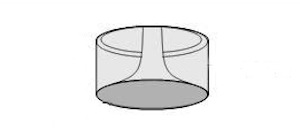
\includegraphics[width=0.5\textwidth]{valve_curtain.jpg}
  \caption{Área de cortina}
  \label{fig:area_cortina}
\end{figure}

Con la población definida se procede a los evaluar cada motor con la función
objetivo, la cual se definió de manera tal de favorecer curvas de rendimiento
volumétrico suaves y valores altos a mayores RPM.

La suavidad de la curva de rendimiento volumétrico se calcula midiendo los
cambios de pendiente de la derivada la cual se aproxima con la fórmula de
diferencia progresiva \ref{eq:derivada}.
%
Solamente interesa el signo, por lo que el valor de $h$ en el denominador no
interesa y se hace 1, con esto la función objetivo queda como el algoritmo
\ref{alg:funcObj}.

\begin{equation}
  f' = \frac{f(i+1) - u(i)}{h}
  \label{eq:derivada}
\end{equation}


% \begin{algorithm}
%     \caption{Calculo del puntaje de una curva de rendimiento volumétrico [r] de
%     $1xN$ y [w] pesos}\label{alg:funcObj}
%     \SetAlgoLined
%
% \Procedure{Función Objetivo}{$r,w,N$}
%   \State $d\gets 0$\Comment{Aproximación a la derivada de r}
%   \State $p\gets 0$\Comment{Penalidad}
%
%   % Aprox de la derivada
%   \For{$i=1:N$}
%     \State $d[i]\gets r[i+1]-r[i]$
%   \EndFor
%
%   % Calculo de la penalidad
%   \For{$i=1:N-1$}
%     \If{$d[i] \cdot d[i+1] < 0$}
%       \State $p\gets p + 1$
%     \EndIf
%   \EndFor
%   \State $p \gets 1 - \frac{p}{N-1}$
%
%   % Puntaje bruto
%   \State $w \gets 0$\Comment{Puntaje sin penalizar}
%   \For{$i=1:N$}
%     \State $w \gets r[i] \cdot w[i]$
%   \EndFor
%
%   % Puntaje con penalidad
%   \State $s \gets w \cdot p$
%   \State \textbf{return} $s$\Comment{s es el puntaje de la curva de rendimiento
%     volumétrico}
%
% \EndProcedure
% \end{algorithmic}
% \end{algorithm}

El conjunto de pesos utilizados para ponderar los rendimientos es el indicado
en la tabla \ref{tab:pesos}

\begin{table}
  \centering
  \begin{tabular}{rccccccccc} \toprule
      RPM  & $w$ \\ \midrule
      1000 & 1 \\
      2000 & 1 \\
      3000 & 1 \\
      4000 & 6 \\
      5000 & 8 \\
      6000 & 9 \\
      7000 & 8 \\
      8000 & 7 \\
      9000 & 7 \\ \bottomrule
  \end{tabular}
  \caption{Pesos}
  \label{tab:pesos}
\end{table}


Una vez evaluados todos los motores de la población, se debe seleccionar los
individuos que forman la población para la siguiente iteración.
%
El método de selección es de tipo TORNEO, en el cual se seleccionan los mejores
$k$ individuos de un grupo al azar de $N$ candidatos.
%

Con los nuevos candidatos seleccionados, se procede a variar la población,
realizando la cruza y mutación.

Luego se toman pares de individuos y de acuerdo a la probabilidad de cruza, se
combinan con el método seleccionado.

Finalmente se realiza una segunda iteración sobre la nueva población, aplicando
el método de mutación a cada individuo, de acuerdo a la probabilidad de
mutación indicada.


El método de cruza seleccionado es \emph{cruza de dos puntos}, en este método
se corta el vector que forma al individuo en dos puntos, la posición de estos
puntos se selecciona al azar, manteniendo el largo original de los vectores.
%
Luego los individuos ``cruzados'' se combinan de forma complementaria, como en
la figura \ref{fig:cr2puntos}

\begin{figure}
  \centering
  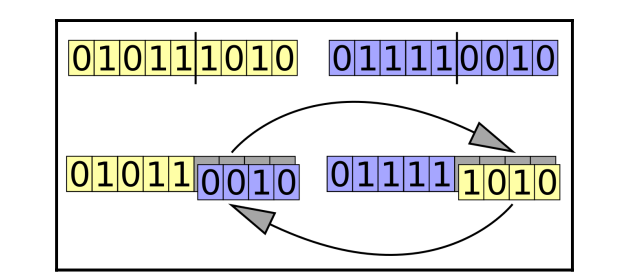
\includegraphics[width=0.5\textwidth]{cruza2puntos.png}
  \caption{Cruza de dos puntos}
  \label{fig:cr2puntos}
\end{figure}

% \begin{algorithm}
% \caption{Cruza de dos punos}\label{alg:c2puntos}
% \begin{algorithmic}[1]
% \Procedure{Cruza}{$a,b,n$}
%
%   \State $i\gets random(1:n)$
%   \State $j\gets random(1:n)$
%
%   % Aprox de la derivada
%   \For{$i=1:N$}
%     \State $d[i]\gets r[i+1]-r[i]$
%   \EndFor
%
%   % Calculo de la penalidad
%   \For{$i=1:N-1$}
%     \If{$d[i] \cdot d[i+1] < 0$}
%       \State $p\gets p + 1$
%     \EndIf
%   \EndFor
%   \State $p \gets 1 - \frac{p}{N-1}$
%
%   % Puntaje bruto
%   \State $w \gets 0$\Comment{Puntaje sin penalizar}
%   \For{$i=1:N$}
%     \State $w \gets r[i] \cdot w[i]$
%   \EndFor
%
%   % Puntaje con penalidad
%   \State $s \gets w \cdot p$
%   \State \textbf{return} $s$\Comment{s es el puntaje de la curva de rendimiento
%     volumétrico}
%   \EndProcedure
% \end{algorithmic}
% \end{algorithm}

El método de mutación seleccioand es mutShuffleIndexes (también podria se
mutFlipBit), en el cual se modifica el orden los números que componen al vector,
dando lugar a por ejemplo:

(figura con ejemplo)

\chapter{Flujometrías}
%
% El simulador ICESym requiere de información sobre el coeficiente de descarga
% (Cd) para simular el flujo a través de los puertos, en trabajos anteriores se
% realizaron simulaciones computacionales del motor con valores de Cd estimados
% \cite{lopez13}.
%
Para obtener una mejor caracterización del funcionamiento de los puertos de
admisión y escape es necesario tener mayor conocimiento del coeficiente de
descarga para diferentes condiciones operativas de los mismos.
%
Se realizaron una serie de flujometrías para obtener un mapa de $C_D$ que sea
función de la diferencia de presión que \emph{ve} el puerto y la apertura del
mismo \footnote{ICESym utiliza alzada, por lo que se traduce área de pasaje de
puerto en alzada de válvula equivalente.}, de modo obtener $C_D = f(\Delta P,L_v)$.
%
Este mapa se usa en ICESym para obtener una simulación más precisa del motor.

Las flujometrías se realizaron con el \emph{software} libre \emph{OpenFoam}, con
los módulos \emph{pimleFoam} para flujo incompresible y y \emph{rhoPimpleFoam}
para flujo compresible.

Para modelar la turbulencia se utilizó un modelo de dos ecuaciones
\emph{$\kappa-\epsilon$}\cite{wilcox}, este es uno de los modelos más utilizados
y, por ser de dos ecuaciones es un modelo completo es decir, provee una ecuación
para $\kappa$ y otra para la escala de longitud turbulenta $l_m$.
%
El modelo requiere que se aproximen los valores iniciales de $\kappa$ y
$\epsilon$, que a su vez requieren de la estimación de la longitud de mezcla o
escala de la viscosidad $l_m$.
%
Los valores iniciales se calculan a partir de:

\begin{align}
    %
    C_{\mu}  &= 0.09 \\
    %
    I        &= 0.05 \\
    %
    l_m      &= 0.07 \cdot D_m \\
    %
    \kappa   &= 1.5 \cdot \left( u_{ref} \cdot I \right) ^ 2 \\
    %
    \epsilon &= \frac{C_\mu ^{3/4} \cdot \kappa ^{3/2}} {l_m}
    %
\end{align}

Dónde:
%
\begin{itemize}
    \item $C_{\mu}$, es un coeficiente propio del modelo.
        %
    \item I, es la intensidad de turbulencia estimada, en este trabajo se utilizó 0.05.
        %
    \item $l_m$, es la longitud de mezcla o escala de viscosidad,
     para flujos internos se suele usar el diámetro hidráulico de la cañería.
        %
    \item $\kappa$, es la energía cinética turbulenta.
        %
    \item $\epsilon$, es la disipación de energía cinética turbulenta.
        %
\end{itemize}

La aproximación de $l_m = D_h$ viene dada porque la longitud de mezcla, que
determina el tamaño que pueden tener los \emph{eddys} turbulentos, puede tomar
valores de orden similar al (nota esto falta)
%
Se utilizo inicialmente el diámetro de la entrada al puerto, en el extremo que
limita con los conductos de admisión o escape, sin embargo el área de pasaje es
menor a la de la boca de los puertos por lo que se decidió utilizar la altura de
cámara, $l_m = h_c$.

%% Esto teniendo en cuneta que para realizar las flujometrías se utiliza el
%% %% algoritmo PIMPLE, el cual se puede utilizar en casos con estimaciones
%% iniciales a las variables viscosas o mal inicializados


\section{Geometria}
Previo a definir otros detalles de las flujometías, es necesario definir alguna
nomenclatura para la geometría, nombre asignado a superficies como paredes,
entrada, salida y cámara de combustión.
%
Para las flujometrías en las que no hay solape de cámaras, se definen las
propiedades de una entrada y una cámara de combustión, indicadas como
\emph{port} y \emph{chamber} respectivamente como se ve en la figura
\ref{fig:ref_geom1}.
%
(Figura aca)

El puerto y la cámara de combustión (o cámaras en caso de que haya solape), se
definen como \emph{patch}, una frontera permeable.
%
El resto de las superficies se definen como paredes \emph{wall}.


\section{Condiciones Iniciales}
%
Las condiciones inicilaes se obtienen de la corrida del simulador obtenida de
la optimización inicial, con coeficientes de descarga constantes.
%
En la tabla \ref{tab:ci} se listan los datos necesarios para las flujometrías
con flujo simulado como incompresibles y compresibles, estos valores se obtienen
a partir de los datos de salida de ICESym para obtener el estado del gas
en la cámara de combustión y límite del puerto correspondiente

(tabla con condiciones inciales)

No se considera la transferencia de calor en las paredes.

Debido a la cantidad de flujometrías a realizar, se utilizó un script para leer los
datos de salida de ICESym y

\section{Coeficiente de descarga ($C_D$)}

El coeficiente másico se calcula a partir de las ecuaciones de flujo
compresible a través de una restricción, para el caso en que el flujo no esté
bloqueado, la ecuación de $\dot{m}$ es:

\begin{equation}
    \label{eq:m_not_choked}
    \dot{m} = \frac{C_D A_R p_0}{\sqrt{R T_0}}
            {\left(\frac{p_T}{p_0} \right)}^{1/\gamma}
            {\left( \frac{2\gamma}{\gamma-1} \left[1- {(\frac{p_T}{p_0})}^{{\gamma-1}/\gamma} \right] \right)} ^{1/2}
\end{equation}

En caso del que el flujo esté bloqueado, es decir
$p_T/p_0 \le [2/\gamma+1)]^{\gamma/(\gamma - 1)}$
, la ecuación correspondiente es:

\begin{equation}
    \dot{m}=  \frac {C_D A_R p_0} {(R T_0)^{1/2}}
            \gamma^{1/2}
            \left( \frac{2\gamma}{\gamma+1} \right)^{(\gamma+1)/(2(\gamma-1))}
\end{equation}

Para determinar $C_D$ se debe conocer:

\begin{itemize}
    \item $p_0$, es la presión de estancamiento antes de la restricción.
    \item $T_0$, es la temperatura de estancamiento antes de la restricción.
    \item $p_T$, es la presión estática justo después de la restricción.
    \item $A_R$, es el área de referencia.
    \item $\dot{m}$, es el caudal másico.
    \item $\gamma$, es el cociente de capacidades térmicas del gas.
\end{itemize}

El área de referencia utilizada en ICESym es el área frontal del puerto expuesta
a la cámara que se esté analizando, caluclada como $A_{R} = h_{p} \cdot l_{{v}}$.
%
Debido a que el MRCVC no tiene válvulas, en trabajos anteriores se confeccionó
un script para calcular la distancia $l_v$ en función del ánuglo del ciclo.
%
En la figura \ref{fig:area_referencia} se ilustran las áreas de referencia para
una posición del rotor en la que hay solape de cámaras con $\theta = 55^\circ$.

\begin{figure}
    \centering
    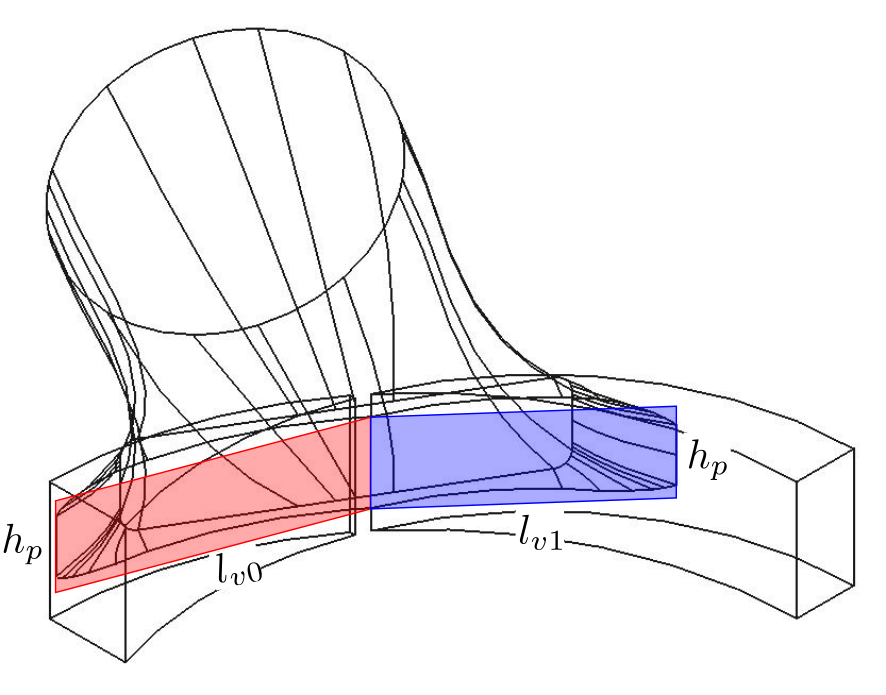
\includegraphics[]{area_referencia.png}
    \caption{Área de referencia}
    \label{fig:area_referencia}
\end{figure}

Los valores de densidad, velocidad, presión y temperatura se obtienen de los
datos de salida de ICESym para un puerto, ángulo y velocidad dada, en
particular del archivo de salida con nombre \emph{$cyl_0.txt$} que contiene
información relevante a la cámara de combustión.
%
Para la temperatura se utiliza la temperatura de cámara, $T_0 = T_C$, la
presión antes y después del puerto se selecciona de acuerdo al sentido de
flujo, en caso de ser flujo hacia la cámara de combustión, la presión en el
puerto se utiliza como inicial $P_0$ y la presión en la cámara es la
aproximación a la presión en la restricción $P_T$.

Para inicializar el campo de presión y densidades, se usa la media entre las
cámaras que se estén simulando y se establerce un campo uniforme.

La velocidad se incicializa con un campo nulo de velocidades, que en la
configuración de OpenFOAM se designa como \emph{internalField uniform (0 0 0)}.

En resumen, los valores iniciales de los campos de presión, temperatura y velocidad

\begin{table}
\centering
    \begin{tabular}{cccc} \toprule
        Var & Campo         & Parche                      & Pared \\
        T   & uniforme T0   & inletOutlet                 & uniforme T9\\ \midrule
        P   & uniform Pavg  & uniformTotalPressure        & Pi \\
        U   & uniform (0 0 0) & pressureInletOutletVelocity & valor fijo(0 0 0)\\
        rho & uniform rhoAvg \\ \bottomrule
    \end{tabular}
    \caption{Condiciones iniciales} \label{tab:cc}
\end{table}

En todos los casos se tomará como velocidad de referencia a la media entre la
velocidad en la punta del tubo de las cámaras solapadas.
%
Del mismo modo, la temperatura será la temperatura de cámara media.

Si hay o no solape de cámaras va a depender tanto de la geometría del puerto
como de la posición del ciclo en la que se encuentre, para determinar las
condiciones iniciales se debe tener en cuenta el solape.
%
En la figura \ref{fig:geom} se muestra un corte del puerto con un plano cuya
normal está en $\vec{z}$, se denominará a la cámara que esté a la izquierda
como cámara 0 y a la que esté a la derecha cámara 1
%
Al haber solape de cámaras, para definir la presión del puerto y estimar las
condiciones iniciales de los parámetros viscosos que requiere el modelo
$k-\epsilon$ se utilizan valores medios de presión, velocidad y temperatura de
ambas cámaras.
%
Además, las condiciones inicales de que se aplican al parche denominado
\emph{puerto} es igual a la media aritmética de la velocidad de las velocidades
de los puertos de ambas cámaras, Lo mismo sucede con la presión, densidad y
temperatura.

A partir de estos datos se calculan varias propiedades termodinámicas del gas,
incluyendo la constante del gas, masa molar, viscosidad cinemática y demás.
%
Para calcular estas propiedades se asume que el gas no contiene gases
residuales.

Finalmente el caudal másico yse obtiene con OpenFOAM, en donde se simula el
tiempo suficiente para que los caudales másicos por entradas o salidas se
estabilice, como se ve en la figura \ref{fig:caudalMasico}.

\begin{figure}
    \centering
    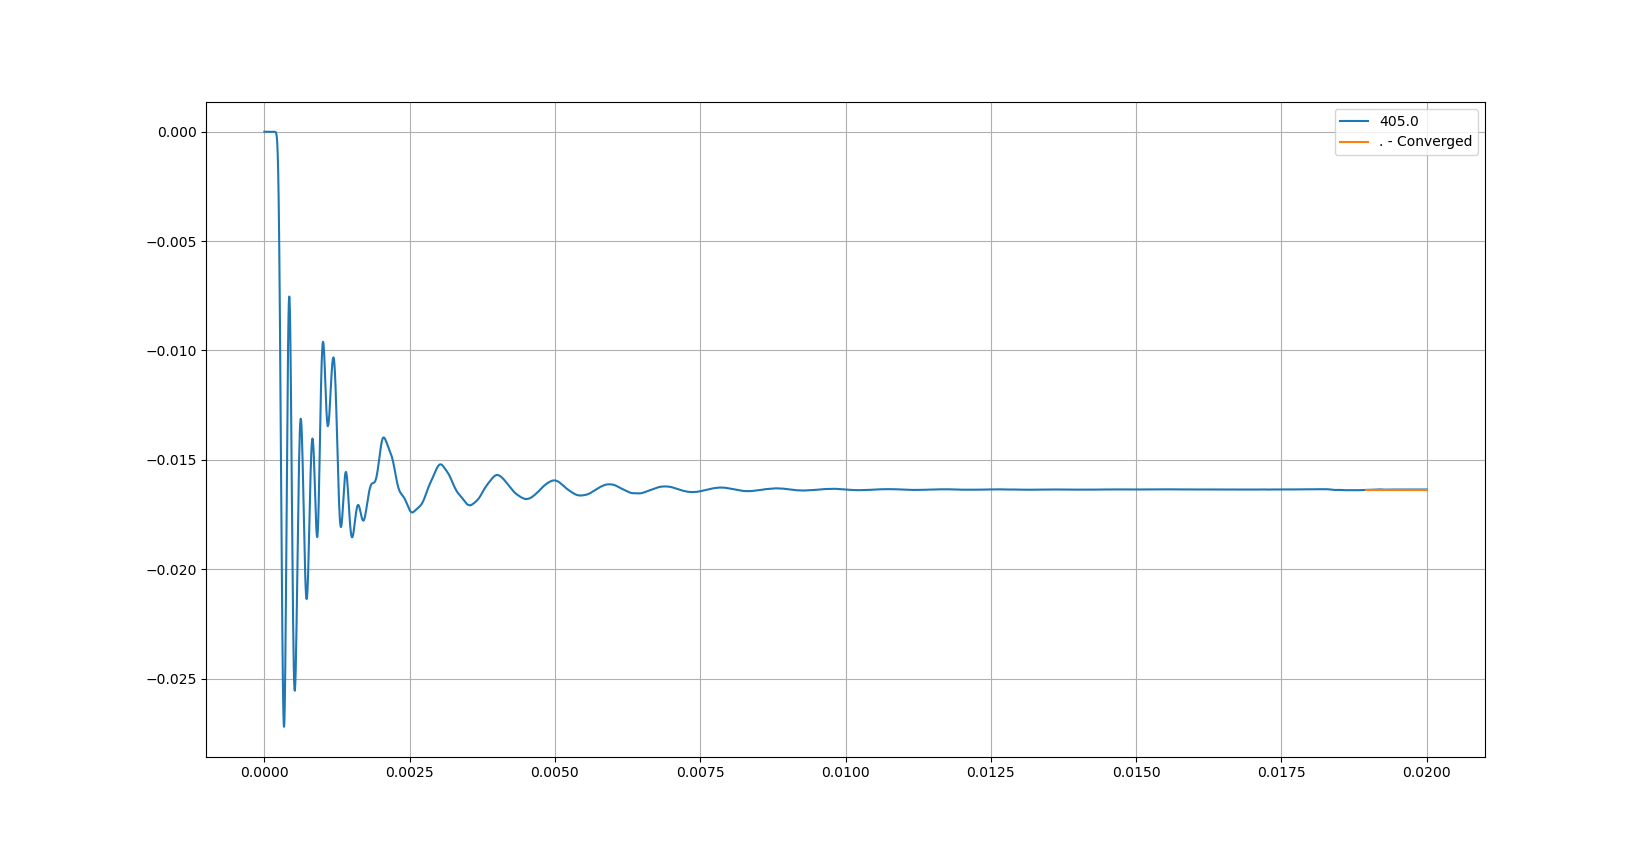
\includegraphics[width=0.6\textwidth]{surfaceFieldValue_405.0.png}
    \caption{Flujometrías para el puerto de Admisión}
    \label{fig:caudalMasico}
\end{figure}
En todos los casos se tomará como velocidad de referencia a la media entre la
velocidad en la punta del tubo de las cámaras que se estén solapando.
%
Del mismo modo, la temperatura será la temperatura de cámara media.

Si hay o no solape de cámaras va a depender tanto de la geometría del puerto
como de la posición del ciclo en la que se encuentre, para determinar las
condiciones iniciales se debe tener en cuenta el solape.
%
En la figura \ref{fig:geom} se muestra un corte del puerto con un plano cuya
normal está en $\vec{z}$, se denominará a la cámara que esté a la izquierda
como cámara 0 y a la que esté a la derecha cámara 1
%
Al haber solape de cámaras, para definir la presión del puerto y estimar las
condiciones iniciales de los parámetros viscosos que requiere el modelo
$k-\epsilon$ se utilizan valores medios de presión, velocidad y temperatura de
ambas cámaras.
%
Además, las condiciones inicales de que se aplican al parche denominado
\emph{puerto} es igual a la media aritmética de la velocidad de las velocidades
de los puertos de ambas cámaras, Lo mismo sucede con la presión, densidad y
temperatura.


\subsection{Mapa de $C_D$}
%
Para obtener el mapa se tomaran valores de flujo másico en las combinaciones de
$(\Delta P, l_v)$ que están indicadas en la tabla \ref{tab:casos}.
%
% En la figura \ref{fig:flujometrias} se ve que se eligieron más cantidad de
% muestreos en las zonas donde hay mayores cambios de presión.
%
% La figura \ref{fig:flujometrias} fué obtenida a partir de los resultados del
% simulador ICESym, restando para las velocidades seleccionadas la presión de la
% cámara a la presión en la boca del puerto.

\begin{figure}
    \centering
    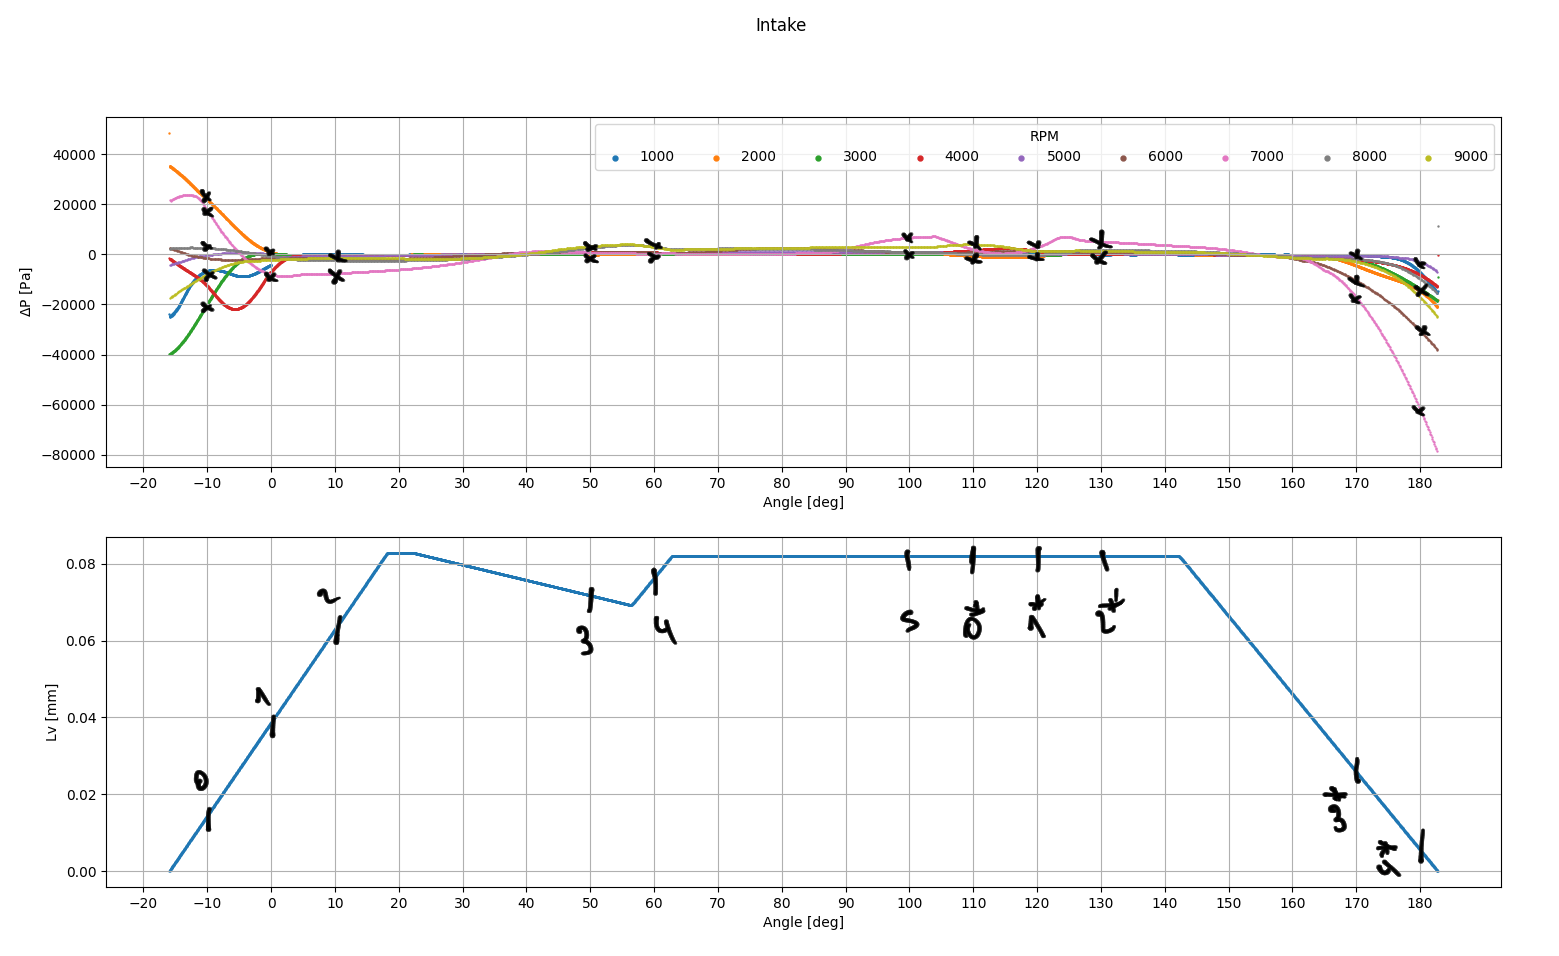
\includegraphics[width=1\textwidth]{flujometrias_admision.png}
    \caption{Flujometrías para el puerto de Admisión}
    \label{fig:flujometrias}
\end{figure}

\begin{table}
    \centering
    \begin{tabular}{rll} \toprule
        Caso & Ángulos  & Velocidades (rpm) \\ \midrule
        0    & -10, 110 & 1000, 2000, 3000, 7000, 8000 \\
        1    & 0, 120   & 2000, 7000 \\
        2    & 10, 130  & 2000, 7000 \\
        3    & 50, 170  & 3000, 7000, 9000 \\
        4    & 60, 180  & 3000, 5000, 6000, 7000 \\
        5    & 95       & 1000, 7000\\ \bottomrule
    \end{tabular}
    \caption{Flujometrías a realizar}
    \label{tab:casos}
\end{table}

Como se ve en la Figura \ref{fig:flujometrias}, los puntos a evaluar son los
listados en la Tabla \ref{tab:casos}.



\begin{figure}[h]
    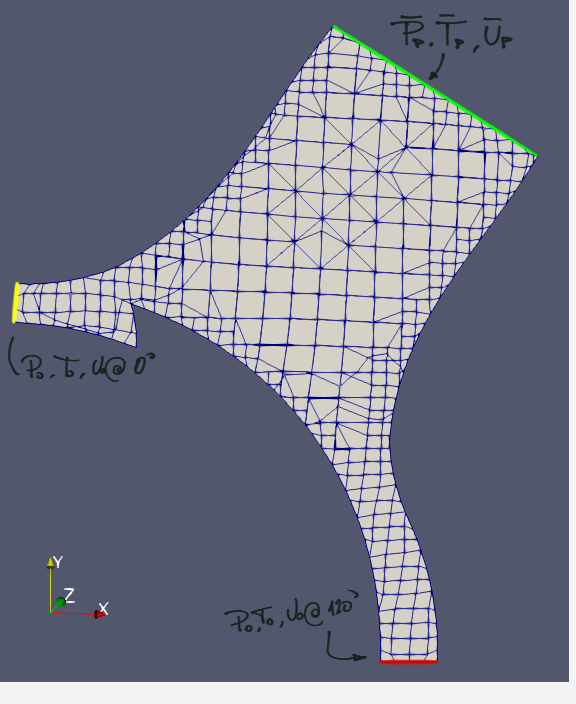
\includegraphics[width=0.8\textwidth]{caso_1-cc.png}
    \caption{Condiciones de borde}
    \label{fig:geom}
\end{figure}

Dentro del volumen de control, el campo de presiones se inicializa con el valor
medio de presiones de las cámaras y el campo de velocidades se hace
inicialmente (0,0,0).

\section{Estudio de convergencia de malla}
%
Para generar la malla primero se representa el volumen a simular con freecad,
procesada con slaome para obtener un conjunto de parches en formato ASCII stl
que puede ser procesado por snappyHexMesh.

snappyHexMesh requiere de una malla inicial para poder comenzar a tabajar, esta
se genera con la aplicaicón blockMesh



%Un estudio de convergencia de malla es una herramienta para evaluar los errores
%de discretización espacial de un estudio de CFD y consiste básicamente en:

%\begin{enumerate}
%    %
%    \item Seleccionar un indicador del tamaño de malla $h$.
%    %
%    \item Elegir un indicador de la convergencia de malla $f$, suele ser la
%        variable de estudio.
%    %
%    \item Seleccionar un coeficiente de refinamiento $r$ y realizar al menos 2
%        simulaciones, manteniendo $r$ constante.
%    %
%    \item Calcular el orden de convergencia de la serie de datos $p$.
%    %
%    \item Estimar $f_{h=0}$
%    %
%    \item Calcular el Índice de Convergencia de Malla (GCI por sus siglas en
%        inglés).
%    %
%    \item Comprobar que se está dentro del rango asintótico de convergencia.
%    %
%\end{enumerate}

%El error de discretización surge de aplicar las ecuaciones de gobierno a un
%dominio espacial discreto (la malla).
%%
%A medida que se reduce el tamaño de celda, el resultado del estudio de CFD se
%vuelve menos sensible a mayores refinamientos y es esperable que el error de
%discretización tienda asintóticamente a cero cuando el tamaño de la malla
%tiende a cero.

%En la Figura \ref{fig:flujometrias} y la Tabla \ref{tab:casos} se indican los
%puntos donde se va a ensayar el puerto de admisión con el fin de obtener el
%valor de caudal másico o volumétrico que fluja por el puerto en distintas
%posiciones del rotor y a distintas velocidades de rotación.
%%
%Dada la cantidad de flujometrías a realizar se opta por realizar el estudio de
%convergencia solo en algunos de los casos, los cuales serán utilizados como
%referencia e indicarán el nivel mínimo de refinamiento mínimo necesario a
%utilizar para todos los casos.

%% Se utilizará el mismo paso tempral en todos los refinamientos.

%\begin{sidewaysfigure}
%    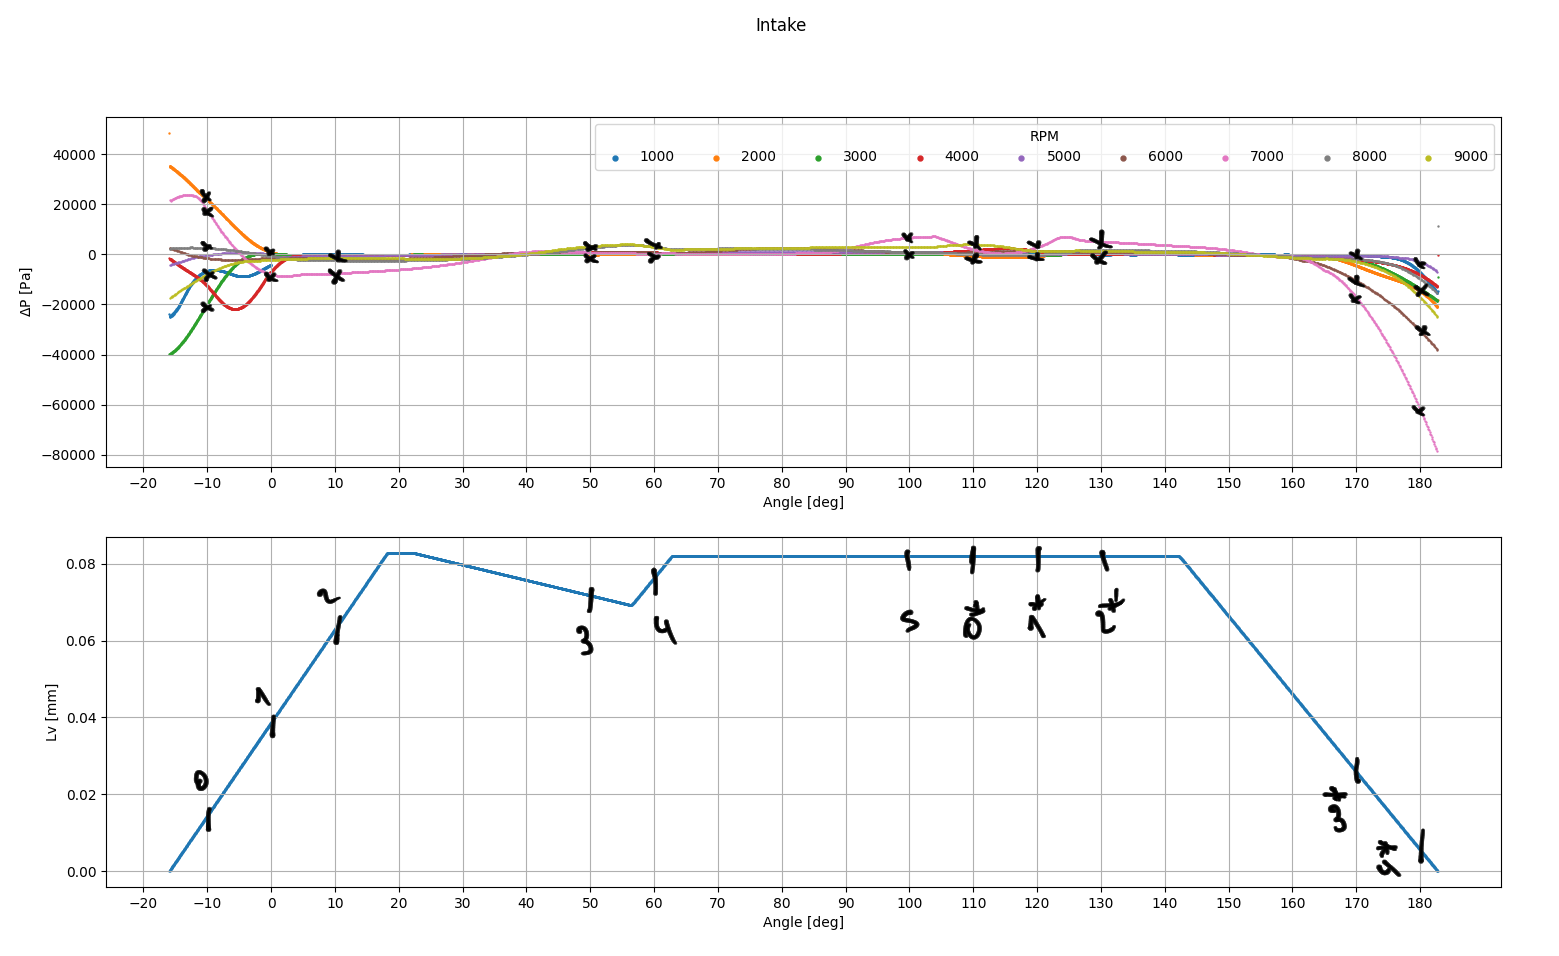
\includegraphics[width=1\textwidth]{flujometrias_admision.png}
%    \caption{Flujometrías para el puerto de admisión}
%    \label{fig:flujometrias}
%\end{sidewaysfigure}

%\begin{table}
%    \centering
%    \begin{tabular}{rcc} \toprule
%        Caso & Ángulos & Velocidades (rpm) \\ \midrule
%        0 & -10, 110 & 1000, 2000, 3000, 7000, 8000\\
%        1 & 0, 120 & 2000, 7000\\
%        2 & 10, 130 & 2000, 7000\\
%        3 & 50, 170 & 3000, 7000, 9000\\
%        4 & 60, 180 & 3000, 5000, 6000, 7000\\
%        5 & 95 & 1000, 7000\\ \bottomrule
%    \end{tabular}
%    \caption{Flujometrías para el puerto de admisión}
%    \label{tab:casos}
%\end{table}

%Hay que distinguir en entre los refinamientos necesarios de flujometrías en
%régimen compresible e incompresible, los casos a tomar como referencia son el
%0, 4 y 5.

%\subsection{Selección de $h$, $r$ y $f$}
%%
%El procedimiento para generar la malla consiste en crear una malla inicial con
%la utilidad \emph{blockMesh} la cual es un punto de partida de
%\emph{snappyHexMesh}.
%%
%Se busca que la malla creada por \emph{blockMesh} este compuesta por celdas
%cúbicas, como se ilustra en la Figura \ref{fig:celdas_bm} el lado de estas
%celdas es el que se toma como indicador del tamaño de malla $h$.
%%
%El coeficiente de refinamiento es el cociente entre el tamaño $h$ de dos pasos
%de refinamiento, como se indica en la ecuación \ref{eq:r}, el mismo se toma
%igual a 1.5 y se mantiene constante para todos los refinamientos.
%%
%Se realizarán refinamientos con mallas de $11.25mm \rightarrow 7.5mm
%\rightarrow 5mm$.

%\begin{equation}
%    \label{eq:r}
%    r = \frac{h_{i+1}}{h_{i}} = 1.5
%\end{equation}


%\begin{figure}[h]
%    \centering
%    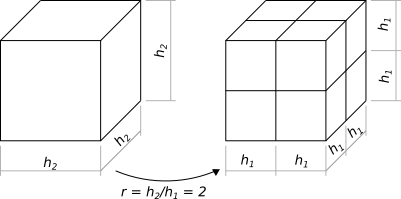
\includegraphics{celdas_block_mesh.png}
%    \caption{Refinamiento con $r=2$}
%    \label{fig:celdas_bm}
%\end{figure}

%Para verificar la convergencia de malla se utiliza el flujo másico a través
%de las superficies definidas como entrada/salida de cámaras.
%%
%En la figura \ref{fig:parches} se indican las superficies por las cuales hay
%flujo másico, siempre que haya solape de cámaras, la cámara que esté a la
%izquierda será llamada cámara 0 y la que esté a derecha cámara 1.
%%
%La superficie que indica la conexión entre el puerto y el resto de los conductos
%de intercambio de gases se denominará puerto.


%En caso de flujo presente un $Ma < 0.3$, el \emph{solver} a utilizar devuelve
%el flujo volumétrico, por lo que se usa este como indicador en lugar del flujo
%másico.

%\begin{figure}[ht]
%    \centering
%    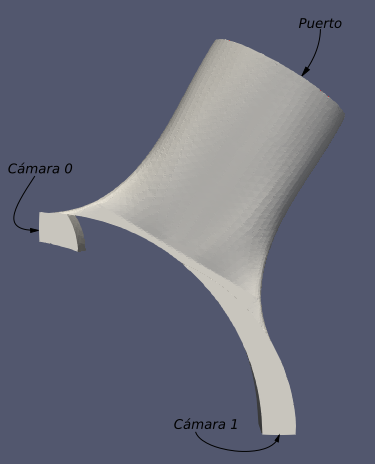
\includegraphics[width=0.4\textwidth]{nombres-parches.png}
%    \caption{Vista superior del volumen de control}
%    \label{fig:parches}
%\end{figure}

%\subsection{Orden de convergencia}
%%
%El orden de convergencia $p$ indica que tan rápido se acerca una secuencia a un
%límite.
%%
%Una secuencia ${x_n}$ que converge a $x^*$ tiene orden de convergencia $p \ge
%1$ y constante asintótica de error $\mu$.

%\begin{equation}
%    \lim_{n\rightarrow \infty} \frac{|x_{n+1} - x^*|} {|x_{n} - x^*|^p} = \mu
%\end{equation}

%El orden de convergencia se puede obtener de comparando el comportamiento del
%error, definido como la diferencia ente la solución exacta o del continuo y la
%discreta.

%\begin{equation}
%    E = f(h) - f_{exacta} = Ch^p + \xi
%    \label{eq:1}
%\end{equation}

%Dónde $C$ es una constante, $h$ es una medida del nivel de refinamiento de la
%malla, $p$ es el orden de convergencia y $\xi$ son términos de orden superior.
%%
%Despreciando los términos de orden superior $\xi$ y tomando logaritmo a ambos
%lados, se puede expresar la ecuación \ref{eq:1} como:

%\begin{equation}
%    \log(E) = \log(C) + p \cdot \log(h)
%\end{equation}

%De esta forma $p$ es la pendiente de la curva de $\log(E)=f(\log(h))$ y
%conociendo al menos 3 puntos puede calcular $p$ como:

%\begin{equation}
%p = \ln \left( \frac{ f_3 - f_2 } { f_2 - f_1 } \right) / \ln(r)
%\label{eq:ord-conv}
%\end{equation}

%\subsection{Resultado ''exacto``}
%%
%El resultado de una simulación numérica se puede expresar de forma general
%como:

%\begin{equation} \label{eq:expansion}
%    f = f_{h=0} + g_1 h + g_2 h^2 + g_3 h^3 + ...
%\end{equation}

%Dónde $h$ es el tamaño de la malla y $g_1$, $g_2$ y $g_3$ son funciones
%independientes $h$, la cantidad $f$ es considerada de segundo orden si $g1 =
%0$.
%%
%El valor de $f_{h=0}$ es el resultado que tendría la simulación con una malla
%infinitamente fina, $h \rightarrow 0$.

%\section{Índice de convergencia de malla}
%%
%El índice de convergencia de malla o GCI por sus siglas en inglés es una forma
%de reportar los resultados de convergencia de malla, es un indicador de qué tan
%lejos se encuentran los resultados obtenidos del resultado numérico exacto
%($f_{h=0}$) y surge de la siguiente ecuación:

%\begin{equation} \label{eq:gci}
%GCI_{i \rightarrow j} = \frac{F_S |\epsilon|}{r^p - 1}
%\end{equation}

%Dónde:
%\begin{description}
%    \item[$F_S$] es un factor de seguridad, se toma 1.25.
%    \item[$\epsilon$] es el error relativo $\epsilon = (f_i - f_j) / f_j$
%    \item[$r$] es el factor de refinamiento $r = h_i/h_j$
%    \item[$p$] es el orden de convergencia relativo a los pasos i, j
%\end{description}

%De este modo, si para un nivel de refinamiento $h_i$ la simulación da como
%resultado un valor $x_i$ con $GCI_i$ dado, se puede decir que el resultado
%de la simulación es $x_i \pm GCI_i \cdot 100$.
%%
%Se tomará como GCI aceptable o banda de error un valor cercano a 5\%.

\section{Resultados}

Para determinar el tipo de \emph{solver} a utilizar se hace una primer corrida
de cada caso asumiendo que el flujo se puede asumir como incompresible, es
decir, que el número de Mach máximo del caso convergido va a ser menor a 0.3.
%
Estos resultados no son definitivos en cuanto al \emph{solver} a utilizar,
puede suceder que a medida que refine un caso el $Ma$ aumente, en cuyo caso
se deberá evaluar si es necesario revisar la hipótesis de flujo incompresible.

% ESe dice que el caso converge cuando el flujo másico a través de cualquiera de
% las entradas/salidas del dominio se estabiliza.

El caso se ejecuta hasta obtener una convergencia del caudal másico para todas
las cámaras involucradas en la simulación, inicialmente este tiempo es de 0.01
segundos.
%
El objetivo de cada flujometría es obtener un valor de caudal másico, para esto
se modelo cada puerto en distintas posiciones y velocidades de rotación.
%
Como se mencionó,los valores iniciales se determinan a partir de los datos de
salida del simulador, con un script de nombre \emph{pre.py} que es un compilado
de funciones para determinar propiedades termodinámicas de las mezclas de gases
quemados o no quemados.

Con esto se obtiene un mapa de caudales másicos que se utilizan para calcular
el coeficiente de descarga con el uso de un script de nombre \emph{post.py}.


En las imágenes que siguen se muestan el campo de velocidades de un corte de
algunos puntos del mapa obtenido.


El mapa de $C_D$ es un conjunto finito de puntos, estos se utilizan para crear
una superficie mediante el método de interpolación de punto más cercano con
suavizamiento.

Los puntos obtenidos se listan en la tabla xxx y la superficie correspondiente
en la figura xxx.

\begin{table}
    \centering
    \begin{tabular}{rll}\toprule
        Caso & Velocidad [RPM] & $Ma_{max}$ \\ \midrule
        0 & 1000 & 0.29 \\
        0 & 2000 & 0.65 \\
        0 & 3000 & 0.49 \\
        0 & 7000 & 0.65 \\
        0 & 8000 & 0.23 \\
        1 & 2000 & 0.14 \\
        1 & 7000 & 0.4 \\
        2 & 2000 & 0.1 \\
        2 & 7000 & 0.43 \\
        3 & 3000 & 0.16 \\
        3 & 7000 & 0.37 \\
        3 & 9000 & 0.24 \\
        4 & 3000 & 0.35 \\
        4 & 5000 & 0.38 \\
        4 & 6000 & 0.49 \\
        4 & 7000 & 0.63 \\
        5 & 1000 & 0.01 \\
        5 & 7000 & 0.45 \\ \bottomrule
    \end{tabular}
    \caption{Números de Mach}
    \label{tab:mach}
\end{table}

\section{Caso 0 - 1000rpm}

El caso simulado tiene solape de cámaras, una a $-10^{\circ}$ y otra a
$110^{\circ}$, con el motor girando a 1000 RPM.
%
El flujo se modela como incompresible\footnote{Ver Tabla \ref{tab:mach}}, la
geometría del caso y la ubicación de los parches correspondientes a la cámara
0, 1 y a la "boca" del puerto.

\begin{figure}
    \centering
    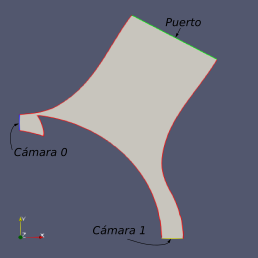
\includegraphics{caso0.png}
    \caption{Geometría a modelar}
    \label{fig:caso0}
\end{figure}

\begin{table}
    \centering
    \begin{tabular}{rll}\toprule
        Parámetro & Valor \\ \midrule
        $\theta_0\ [^{\circ}]$ & 590 \\
        $\theta_1\ [^{\circ}]$ & 110 \\
        $\epsilon_{est}$ & 195.467 \\
        $\gamma_{est}$ & 1.309 \\
        $\kappa_{est}$ & 1.364471 \\
        $\nu_{est}$ & 4.3e-05 \\
        $p_0 [Pa]$ & 107355.2 \\
        $p_1 [Pa]$ & 100867.47 \\
        $\overline{p} [Pa]$ & 104111.33 \\
        $\overline{p_{puerto}} [Pa]$ & 100780.23 \\
        $\overline{\rho} [kg/m^3]$ & 0.643938 \\
        $\overline{T} [K]$ & 589.89 \\ \bottomrule
    \end{tabular}
    \caption{Valores iniciales}
    \label{tab:caso0_ci}
\end{table}


En la tabla \ref{tab:res_caso0}se muestran los resultados de 3 pasos de
refinamiento. TENGO QUE REHACER TODOS EN RÉGIMEN COMPRESIBLE

\begin{table}
    \centering
    \begin{tabular}{rccccc}\toprule
        h [mm] & $h_{norm}$ & $N^{\circ}$ celdas & $Ma$ & $\dot{V_{0}}\ [m^3/s] $ & $\dot{V_{1}}\ [m^3/s]$ \\ \midrule
        5      & 1.0        & 167900             & 0.36 & -0.006312     & -0.012329 \\
        10     & 2.0        & 52210              & 0.33 & -0.006455     & -0.011692 \\
        20     & 4.0        & 20795              & 0.29 & -0.006668     & -0.011652 \\ \bottomrule
    \end{tabular}
    \caption{Flujos volumétricos para ambas cámaras}
    \label{tab:res_caso0}
\end{table}

Con estos datos se puede calcular el orden de convergencia y el resultado
extrapolado a $h=0$.

\begin{table}
    \centering
    \begin{tabular}{rcc}\toprule
        Parámetro & Cámara 0  & Cámara 1  \\ \midrule
        p         &  0.565833 & -3.967099 \\
        $f_{h=0}$ & -0.006013 & -0.011649 \\ \bottomrule
    \end{tabular}
    \caption{Orden de convergencia y resultado exacto}
    \label{tab:res1_caso0}
\end{table}

Y con el orden de convergencia se pueden calcular los valores de GCI.

\begin{table}
    \centering
    \begin{tabular}{rccc}\toprule
        Paso              & $r$ & $GCI_0(\%)$ & $GCI_1(\%)$ \\ \midrule
        1 $\rightarrow$ 2 & 2   & -5.923628   & 6.895404 \\
        2 $\rightarrow$ 3 & 2   & -8.573288   & 0.464910 \\ \bottomrule
    \end{tabular}
    \caption{GCI}
    \label{tab:gci_caso_0}
\end{table}

Con estos resultados se verifica que se esté en rango de convergencia
asintótica, como se indica en la Tabla \ref{tab:rac_caso_0}, los flujos
másicos de ambas cámaras se encuentran en rango de convergencia asintótica.

\begin{table}
    \centering
    \begin{tabular}{rccc}\toprule
        Rango               & $rac_0$  & $rac_1$ \\ \midrule
        12 $\rightarrow$ 23 & 1.022758 & 0.948364 \\ \bottomrule
    \end{tabular}
    \caption{Verificación de convergencia}
    \label{tab:rac_caso_0}
\end{table}


\section{Caso 0 - 7000 rpm}

\section{Caso 4 - 7000 rpm}

\section{Caso 5 - 1000rpm}

El caso simulado tiene una sola cámara a $100^{\circ}$ del ciclo, con el motor
girando a 1000 RPM.
%
El flujo se modela como incompresible\footnote{Ver Tabla \ref{tab:mach}}, la
geometría del caso y la ubicación de los parches correspondientes a la cámara
0, 1 y a la "boca" del puerto.

\begin{figure}
    \centering
    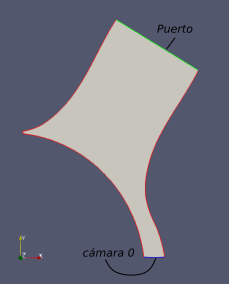
\includegraphics{caso5.png}
    \caption{Geometría a modelar}
    \label{fig:caso5}
\end{figure}

\begin{table}
    \centering
    \begin{tabular}{rll}\toprule
        Parámetro & Valor \\ \midrule
        $\theta_0\ [^{\circ}]$ & 100 \\
        $\epsilon_{est}$ & 25.271765 \\
        $\gamma_{est}$ & 1.329 \\
        $\kappa_{est}$ & 0.348878 \\
        $\nu_{est}$ & 2.9e-05 \\
        $\overline{p} [Pa]$ & 103732.67 \\
        $\overline{p_{puerto}} [Pa]$ & 103773.09 \\
        $\overline{\rho} [kg/m^3]$ & 0.797554 \\
        $\overline{T} [K]$ & 453.18 \\ \bottomrule
    \end{tabular}
    \caption{Valores iniciales}
    \label{tab:caso5_ci}
\end{table}

En la tabla \ref{tab:res_caso5} se muestran los resultados de 3 pasos de
refinamiento.

\begin{table}[h]
    \centering
    \begin{tabular}{rcccc}\toprule
        h [mm] & $h_{norm}$ & $N^{\circ}$ celdas & $Ma$ & $\dot{V}\ [m^3/s]$ \\ \midrule
        5      & 1.0        & 167900             & 0.36 & -0.006312 \\
        10     & 2.0        & 52210              & 0.33 & -0.006455 \\
        20     & 4.0        & 20795              & 0.29 & -0.006668 \\ \bottomrule
    \end{tabular}
    \caption{Flujos volumétricos para ambas cámaras}
    \label{tab:res_caso5}
\end{table}

Con estos datos se puede calcular el orden de convergencia y el resultado
extrapolado a $h=0$.

\begin{table}[h]
    \centering
    \begin{tabular}{rc}\toprule
        Parámetro & Cámara 0  \\ \midrule
        p         &  0.565833 \\
        $f_{h=0}$ & -0.006013 \\ \bottomrule
    \end{tabular}
    \caption{Orden de convergencia y resultado exacto}
    \label{tab:res1_caso5}
\end{table}

Y con el orden de convergencia se pueden calcular los valores de GCI.

\begin{table}
    \centering
    \begin{tabular}{rcc}\toprule
        Paso              & $r$ & $GCI_0(\%)$ \\ \midrule
        1 $\rightarrow$ 2 & 2   & -5.923628   \\
        2 $\rightarrow$ 3 & 2   & -8.573288   \\ \bottomrule
    \end{tabular}
    \caption{GCI}
    \label{tab:gci_caso_5}
\end{table}

\begin{table}
    \centering
    \begin{tabular}{rccc}\toprule
        Rango               & $rac_0$  \\ \midrule
        12 $\rightarrow$ 23 & 1.022758 \\ \bottomrule
    \end{tabular}
    \caption{Verificación de convergencia}
    \label{tab:rac_caso_5}
\end{table}

Con estos resultados se verifica que se esté en rango de convergencia
asintótica, como se indica en la Tabla \ref{tab:rac_caso_5}, los flujos
másicos de ambas cámaras se encuentran en rango de convergencia asintótica.


\section{Mapa de $C_D$}
%
El mapa de $C_D$ obetnido a partir de las flujoemtrías se lista en la tabla
\ref{tab:mapaAdm} y \ref{tab:mapaEsc} para los mapas de admisión y escape
respectivamente.


\begin{table}
  \parbox{.45\linewidth}{
  \centering
  \begin{tabular}{rccc}\toprule
    Item & $L_v[m]$ & $\Delta P[Pa]$ & $C_D$ \\ \midrule
    \lua{tex.print(mapaCd(myData.admision))}
    \bottomrule
    \end{tabular}
  \caption{Mapa $C_D$ del puerto de Admisión}
  \label{tab:mapaAdm}
  }
\hfill
\parbox{.45\linewidth}{
  \centering
  \begin{tabular}{rccc}\toprule
    Item & $L_v[m]$ & $\Delta P[Pa]$ & $C_D$ \\ \midrule
    \lua{tex.print(mapaCd(myData.escape))}
    \bottomrule
    \end{tabular}
  \caption{Mapa $C_D$ del puerto de Escape}
  \label{tab:mapaEsc}
}
\end{table}


\chapter{Resultados}

\section{Introducción}
%
Los resultados obtenidos en cada uno de los pasos de este trabajo se detallan en
este capítulo, comenzando por el motor obtenido en la primer iteración de
optimización con el algoritmo genético, luego se presenta el modelo de CAD
generado para la segunda etapa de simulación.

Luego se muestran los resultados de las flujometrías realizadas con la geometría
obtenida, incluyendo las mallas obtenidas para algunos casos seleccionados y el
resultado detallado de algunas de las flujometrías, finalizando con el mapa de
coeficientes de descarga obtenido, tanto para el puerto de admisión como para el
puerto de escape.

Por último se presentan los resultados de la segunda ronda de optimización con
el algoritmo genético, en la que se utilizó el mapa de coeficientes de descarga
obtenido en el paso previo.
%
En esta sección se muestra además el modelo de CAD generado para esta geometría.

\section{Primer Iteración}
%
La primer optimización se realizó partiendo de una población al azar, con los
coeficientes de descarga constantes de 0.7 y 0.75 para el puerto de admisión y
escape respectivamente.
%
El algoritmo genético se ejecutó durante 100 generaciones con una población de
100 individuos, la función objetivo es la definida en la sección xxx con los
pesos indicados, los operadores y parámetros correspondientes indicados en la
tabla~\ref{tab:config_genetico}.

\begin{table}
  \centering
  \begin{tabular}{cc} \toprule
    Parámetro & Valor \\ \midrule
    RPMS & $(1000, 2000, 3000, 4000, 5000, 6000, 7000, 8000, 9000)$ \\
    Pesos de función objetivo & $(1, 1, 1, 6, 8, 9, 8, 7, 7)$ \\
    Cantidad de ciclos de ICESym & 2 \\
    Diámetro mínimo & 0.05 \\
    Diámetro máximo & 0.1 \\
    Longitud mínima de tubo & 0.5 \\
    Longitud máxima de tubo & 2 \\
    Ángulo mínimo & 0 \\
    Ángulo máximo & 90 \\
    Separación angular máxima & 70 \\
    Tamaño de población & 100 \\
    Tamaño de torneo & 10 \\
    $\mu$ & 0 \\
    $\sigma$ & 1 \\
    $\alpha$ & 0.5 \\
    Probabilidad de cruza & 0.9 \\
    Probabilidad de mutación & 0.5 \\
    Cantidad de generaciones & 20 \\
    Tamaño de \emph{SALÓN DE LA FAMA} & 1 \\ \bottomrule
    \end{tabular}
  \caption{Configuración utilizada.}\label{tab:config_genetico}
\end{table}


En la gráfica de evolución de la aptitud media y máxima de la población se ve
que se obtuvo rápidamente un individuo con un puntaje relativamente alto en la
generación X, un X porciento mayor a la media.
%
El resultado final tiene una aptitud XX mayor a la aptitud media de la
población, los parámetros que definen este candidato son los listados en la
tabla y se ilustran en la figura~\ref{fig:pop_ev_1}.
%
Este motor tiene un rendimiento volumétrico máximo de 0.8 para 1000 rpm y si
bien la función objetivo favorece curvas suaves, se ven dos picos de rendimiento
en la curva, siendo el segundo a 1100 rpm.

\begin{figure}
    \centering
    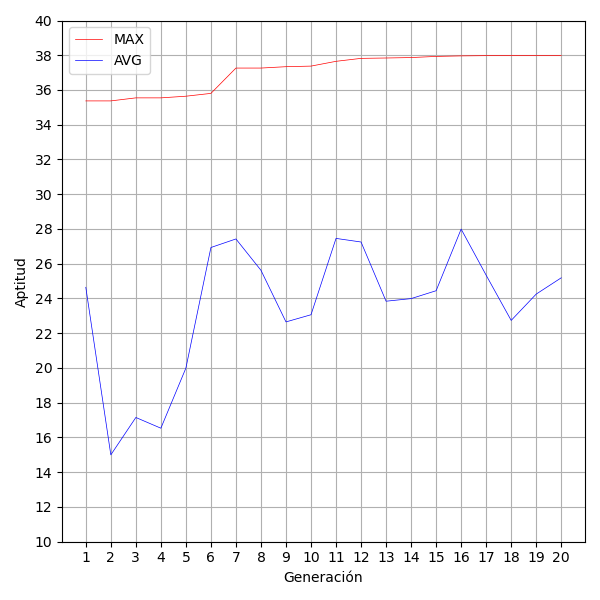
\includegraphics[width=.7\textwidth]{genetico/pop_evolution.png}
    \caption{Evolución de la primer optimización.}\label{fig:pop_ev_1}
\end{figure}

\begin{table}
  \centering
  \begin{tabular}{cc} \toprule
    Parámetro & Valor & Unidad \midrule
    DTA & 97.24 & mm\\
    DTE & 81.15 & mm\\
    LIT & 519.31 & mm\\
    LET & 976.66 & mm\\
    IIA & 1.12 & grado\\
    IFA & 70.15 & grado\\
    EIA & 85.14 & grado\\
    EFA & 11.13 & grado\\ \bottomrule
  \end{tabular}
  \caption{Mejor Candidato.}\label{tab:resultado_primer_it}
\end{table}


En la figura XXX se muestran las curvas de potencia y torque del motor, como es
de esperarse se ve que ambas copian la curva de rendimiento volumétrico, con una
potencia máxima de XXX HP a 1000 rpm y un torque máximo de xxxx N.m. a xxx rpm.

\subsection{Puerto de admisión}

Evaluando las curvas de presión para estas rpm se observa que durante la
apertura del puerto de escape hay una depresión de XXX Pa, para este punto el
coeficiente de descarga se estima en XXX y fluje un XX porciento de la masa
total que ingresa durante el período angular en que se encuentra abierto el
puerto.

El puerto de escape ocupa un período angular de $69^{\circ}$, inciando la
apertura en $1.12^{\circ}$ y cerrando a $70.15^{\circ}$ en relación al giro del
cigüeñal.

Se puede concluir que el puerto de admisión tiene sintonías en XXX, XXX, XXX rpm, siendo los diferenciales de presión mayores en xxx xxx xxx.

\subsection{Puerto de admisión}
%
El puerto de escape ocupa un período angular de $69^{\circ}$, inciando la
apertura en $1.12^{\circ}$ y cerrando a $70.15^{\circ}$ en relación al giro del cigüeñal.


\subsection{Modelo de CAD}
%
Los parámetros geométricos obtenidos se utilizaron para modelar los puertos,
tratando de generar una transición suave entre puerto y cámara de combustión
para favorecer el pasaje de gas.
%
Como se ve en la figura~\ref{fig:motor_cad}, se redondearon las aristas internas incluyendo las
paletas y las puntas del rotor, esto para favorecer el proceso de mallado
requerido en el paso siguiente a este ya que los bordes agudos son complejos de
adaptar a una malla construida con tetraedros, como lo es la malla resultante de
snappyHexMesh que se describió en el apartado xxx del capítulo xxx.

\begin{figure}
  \centering
    \begin{subfigure}{0.4\textwidth}
        \centering
        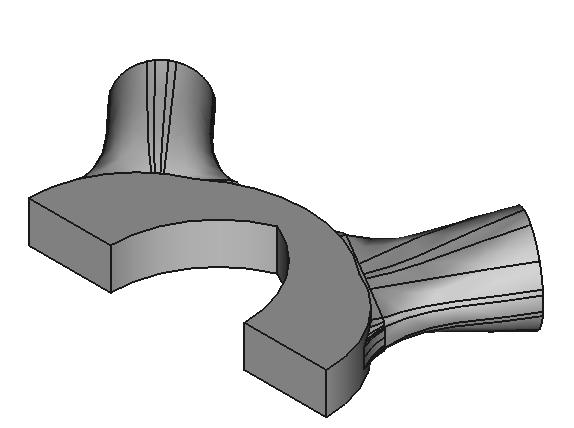
\includegraphics[width=\textwidth]{CAD/motor_cad1.png}
    \end{subfigure}
    \hfill
    \begin{subfigure}{0.4\textwidth}
        \centering
        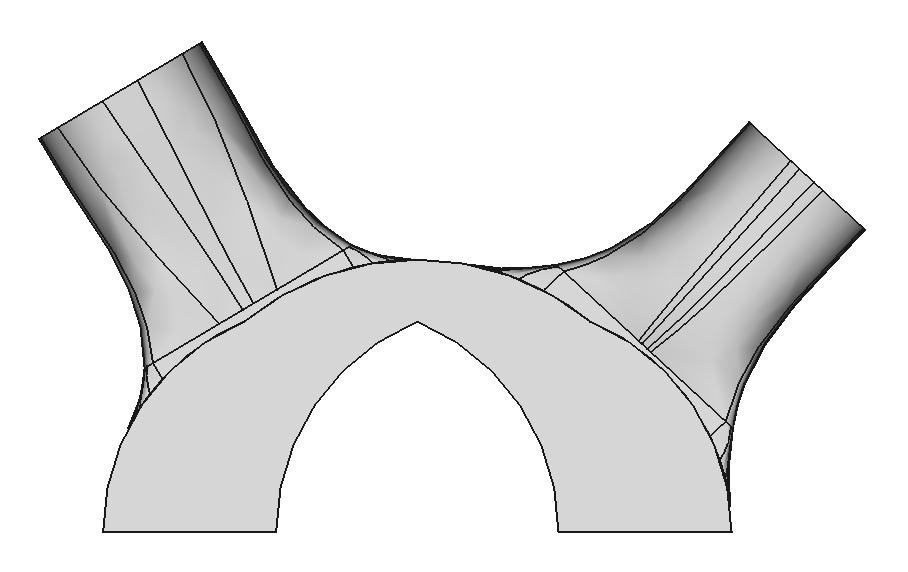
\includegraphics[width=\textwidth]{CAD/motor_cad2.png}
    \end{subfigure}
  \caption{CAD Primer Iteración}\label{fig:motor_cad1}
\end{figure}

La altura del puerto del lado de la cámara de combustión se mantuvo en dos
tercios del a altura de cámara.

\begin{figure}
  \centering
    \begin{subfigure}{0.8\textwidth}
        \centering
        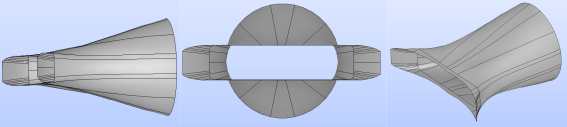
\includegraphics[width=\textwidth]{CAD/vistas_admision.png}
        \caption{Puerto de Admsisión.}
    \end{subfigure}
    \begin{subfigure}{0.8\textwidth}
        \centering
        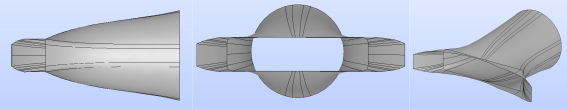
\includegraphics[width=\textwidth]{CAD/vistas_escape.png}
        \caption{Puerto de Escape.}
    \end{subfigure}
  \caption{CAD Primer iteración (vistas fuera de escala).}\label{fig:motor_cad2}
\end{figure}


\section{Flujometrías}

De los resultados de la primer otpimización se extrajo una curva de diferencia
de presión vs alzada para diferentes velocidades del motor para identificar los
puntos de mayor interés para realizar las fluometrías, tratando de obtener una
buena cobertura del rango de funcionamiento de cada puerto.

Inicialmente se propusieron un total de XXX flujometŕias, sin embargo algunas
combinaciones de $\l_{v}, \Delta P$ no se pudieron ejecutar hasta la
convergencia del flujo másico, por lo que se redujo la cantidad de flujometrías
final a xxx flujometrías, xxx para el puerto de admisión y xxx para el puerto de
escape, el par $(\l_{v}, \Delta P)$ se detalla en la figura XXX y tabla xxx.
%
Con estos datos se calculó el coeficiente de descarga para cada punto evaluado
obteniendo la base para generar el mapa de coeficientes de descarga que se
utilizará en el próximo paso de simulación, los valores de presión, alzada y
coeficiente de descarga obtenidos se listan en la tabla xxx.

Como se mencionó en el apartado~\ref{ch:mrcvc}, la modificaión realizada a
ICESym para funcionar con un mapa de $C_{D}$ dependiente de dos variables
requiere que los datos de entrada estén distribuidos en una grilla rectangular,
motivo por el cual a partir de estos valores se utilizó el método de
interpolación por IDW mencionado en el mismo apartado para generar una dicha
grilla de valores de $(l_{v}, \Delta P)$ con $C_{D}$ interpolado de los datos
conocidos, como se ve en las figuras~\ref{fig:mapa_cd_admision}
y~\ref{fig:mapa_cd_escape}.

\begin{figure}
    \centering
    \begin{subfigure}{0.4\textwidth}
        \centering
        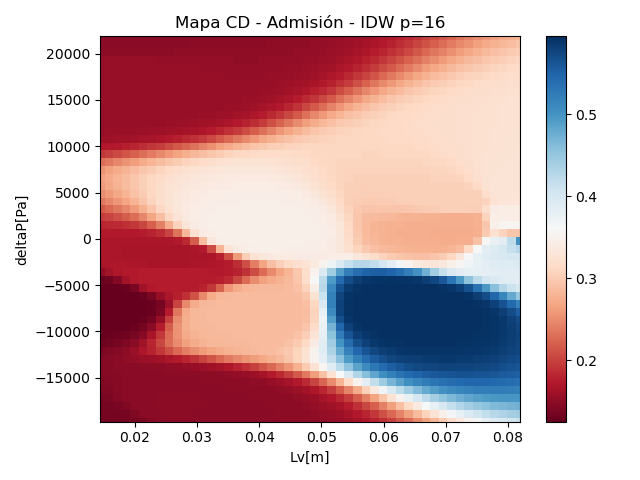
\includegraphics[width=\textwidth]{mapa_cd/idw16_mapa_adm.png}
        \caption{cambiar}
    \end{subfigure}
    \hfill
    \begin{subfigure}{0.4\textwidth}
        \centering
        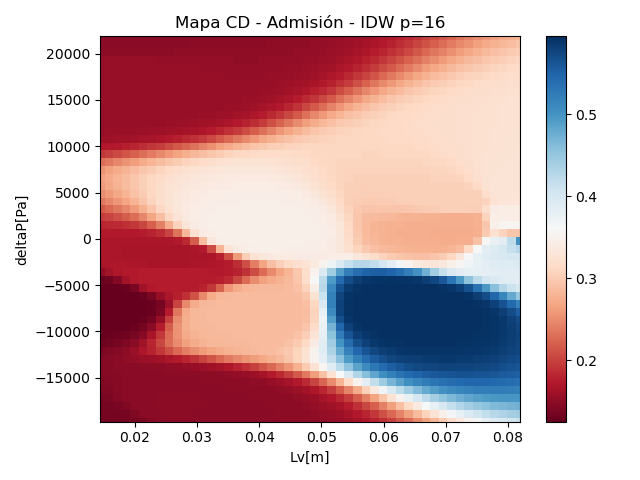
\includegraphics[width=\textwidth]{mapa_cd/idw16_mapa_adm.png}
        \caption{cambiar}
    \end{subfigure}
    \caption{cabmiar}\label{fig:mapa_cd_admision}
\end{figure}

\begin{figure}
    \centering
    \begin{subfigure}{0.4\textwidth}
        \centering
        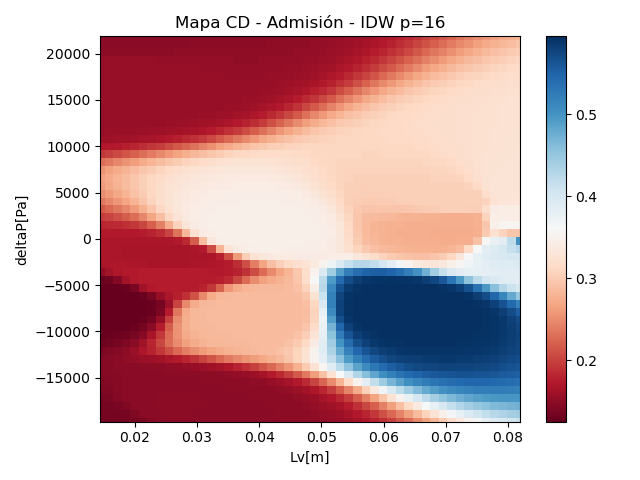
\includegraphics[width=\textwidth]{mapa_cd/idw16_mapa_adm.png}
        \caption{cambiar}
    \end{subfigure}
    \hfill
    \begin{subfigure}{0.4\textwidth}
        \centering
        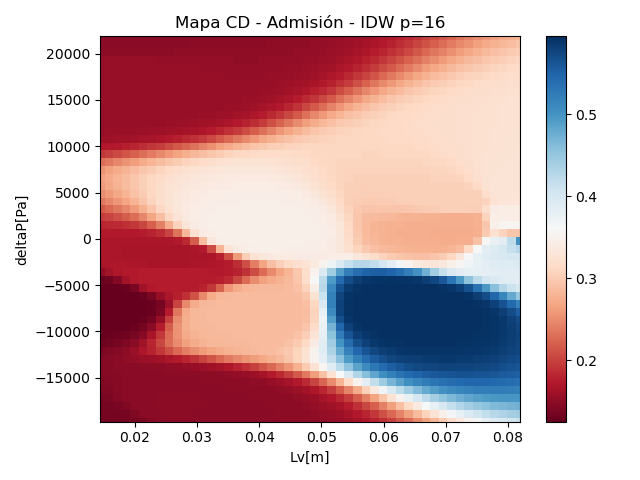
\includegraphics[width=\textwidth]{mapa_cd/idw16_mapa_adm.png}
        \caption{cambiar}
    \end{subfigure}
    \caption{cabmiar}\label{fig:mapa_cd_escape}
\end{figure}

En el mapa del puerto de admisioń se observa un máximo para para aperturas del
puerto mayores a 80mm, con $\Delta P$ de entre 1000 Pa a 15000 Pa.
%
El coefiente de descarga máximo es $C_{D}(100mm, 1500Pa) = 0.6$ y corresponde a
la flujometría $N^{\circ} X$, el flujo másico obtenido para este régimen es de
0.02 kg/s, con un a velocidad máxima de xxx m/s en la garganta.
%
El peor valor se es $C_{D}(100mm, 1500Pa) = 0.6$ y corresponde a aperturas
pequeñas del puerto, en la que debido a la reducida sección de pasaje de flujo
se tiene velocidades eleveadas, siendo la máxima de xxx m/s.
%
Para visualizar la diferencia entre uno y otro caso, se representan las líneas
de corriente para ambos casos en la figura \ref{fig:comparativa_lineas_corriente}.

\begin{figure}
    \centering
    \begin{subfigure}{0.4\textwidth}
        \centering
        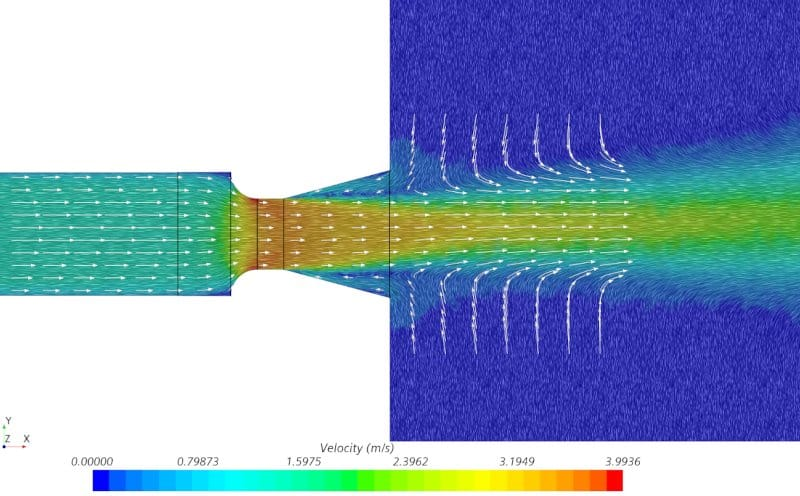
\includegraphics[width=\textwidth]{flujometrias/ejemplo_lineas_corriente.jpg}
        \caption{Valor máximo de $C_{D}$}
    \end{subfigure}
    \hfill
    \begin{subfigure}{0.4\textwidth}
        \centering
        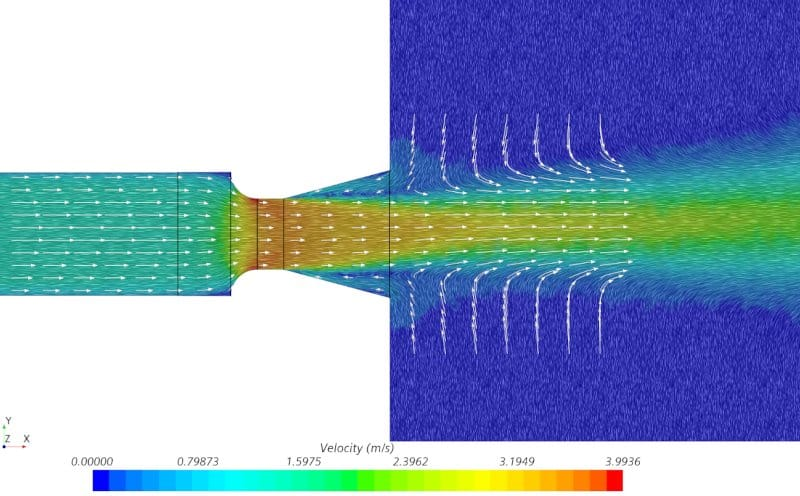
\includegraphics[width=\textwidth]{flujometrias/ejemplo_lineas_corriente.jpg}
        \caption{Valor mínimo de $C_{D}$}
    \end{subfigure}
    \caption{cabmiar}\label{fig:comparativa_lineas_corriente}
\end{figure}

Para el mapa del puerto de escape se observa un máximo para para aperturas del
puerto mayores a 80mm, con $\Delta P$ de entre 1000 Pa a 15000 Pa.
%
El coefiente de descarga máximo es $C_{D}(100mm, 1500Pa) = 0.6$ y corresponde a
la flujometría $N^{\circ} X$, el flujo másico obtenido para este régimen es de
0.02 kg/s, con un a velocidad máxima de 10m/s en la garganta, como se ve en la
figura \ref{fig:admision_10_2000.jpg}.

\begin{figure}
    \centering
    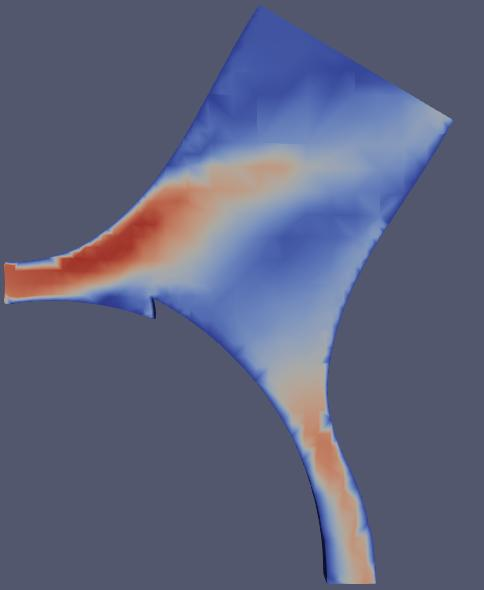
\includegraphics[width=0.7\textwidth]{flujometrias/admision_10_2000.jpg}
    \caption{Puerto de admisión - $10^{\circ}$@2000 RPM}\label{fig:admision_10_2000.jpg}
\end{figure}

El peor valor se es $C_{D}(100mm, 1500Pa) = 0.6$ y corresponde a aperturas
pequeñas del puerto, en la que debido a la reducida sección de pasaje de flujo
se tiene velocidades eleveadas, siendo la máxima de xxx m/s.
%
Para visualizar la diferencia entre uno y otro caso, se representan las líneas
de corriente para ambos casos en la figura \ref{fig:admision_10_2000.jpg}.

\begin{figure}
    \centering
    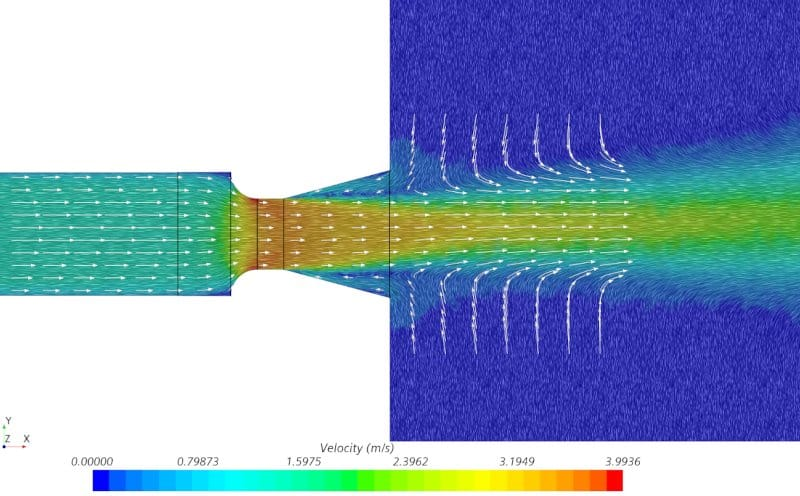
\includegraphics[width=0.7\textwidth]{flujometrias/ejemplo_lineas_corriente.jpg}
    \caption{Puerto de admisión - $10^{\circ}$@2000 RPM}\label{fig:admision_10_2000.jpg}
\end{figure}

En las tablas~\ref{tab:mapa_cd_admision} y~\ref{tab:mapa_cd_escape} se muestran los
resultados de realizar las flujometrías de los puertos de admisión y escape.

\begin{table}
  \centering
    \begin{tabular}{cccc} \toprule
      Caso  & lv        & $\Delta P$    & $C_{D}$   \\ \midrule
      0     & 0.016826  & -100331.39    &  0.213882 \\
      0     & 0.106775  & 5723.72       &  0.489375 \\
      0     & 0.016826  & -263797.72    &  0.011021 \\
      0     & 0.106775  & -3296.18      &  0.803197 \\
      0     & 0.016826  & -652902.78    &  0.011106 \\
      0     & 0.106775  & -9613.29      &  0.815804 \\
      0     & 0.016826  & -513568.73    &  0.011280 \\
      0     & 0.106775  & -3232.97      &  0.813186 \\
      1     & 0.026960  & -116996.12    &  0.375219 \\
      1     & 0.096641  & -3643.9       &  0.878414 \\
      1     & 0.026960  & -237724.11    &  0.018632 \\
      1     & 0.096641  & -6684.11      &  0.867774 \\
      1     &  0.02696  & -496509.46    &  0.111212 \\
      1     &  0.09664  & -18256.20     &  0.805830 \\
      1     & 0.026960  & -237724.11    &  0.022716 \\
      1     & 0.096641  & -6684.11      &  0.862647 \\
      2     & 0.047228  & -49343.47     &  0.541857 \\
      2     & 0.076373  & -5712.86      &  0.918061 \\
      2     & 0.047228  & -109348.67    &  0.487137 \\
      2     & 0.076373  & -17090.38     &  0.914182 \\
      3     & 0.067496  & 13.83         &  0.696967 \\
      3     & 0.071759  & -134.24       &  0.707263 \\
      3     & 0.067496  & -100073.52    &  0.731100 \\
      3     & 0.071759  & -24077.34     &  0.723965 \\
      4     & 0.075750  & -11793.31     &  0.946392 \\
      4     & 0.087764  & -33418.12     &  0.235717 \\
      4     & 0.087764  & -10715.70     &  0.221632 \\
      4     & 0.075750  & -5167.81      &  0.897169 \\
      6     & 0.123601  & -73.94        &  0.878522 \\ \bottomrule
    \end{tabular}
  \caption{Mapa de Cd del puerto de escape} \label{tab:mapa_cd_escape}
\end{table}

\begin{table}
  \centering
  \begin{tabular}{cccc} \toprule
      Caso  & lv        & $\Delta P$    & $C_{D}$   \\ \midrule
      0     & 0.014432  & -6574.97      &  0.206543 \\
      0     & 0.081937  & -87.24        &  0.828822 \\
      0     & 0.014432  & 21856.29      &  0.243975 \\
      0     & 0.081937  & -573.65       &  0.738459 \\
      0     & 0.014432  & -19738.67     &  0.222406 \\
      0     & 0.081937  & 519.60        &  0.487115 \\
      0     & 0.081937  & 1571.95       &  0.587277 \\
      0     & 0.014432  & 18077.97      &  0.256415 \\
      0     & 0.014432  & 2668.61       &  0.247292 \\
      0     & 0.081937  & 0.98          &  0.025970 \\
      2     & 0.062951  & -297.79       &  0.816487 \\
      2     & 0.081937  & 292.92        &  0.466147 \\
      2     & 0.062951  & -7374.88      &  0.980617 \\
      2     & 0.081937  & 4953.85       &  0.541619 \\
      3     & 0.071763  & 4092.13       &  0.501641 \\
      3     & 0.025832  & -3689.81      &  0.289852 \\
      4     & 0.069767  & -789.00       &  0.615690 \\
      4     & 0.069767  & 7869.92       &  0.599348 \\
      4     & 0.005564  & -12539.15     &  0.534555 \\
      4     & 0.005564  & -10091.84     &  0.583979 \\ \bottomrule
    \end{tabular}
  \caption{Mapa de Cd del puerto de Admisión} \label{tab:mapa_cd_admision}
\end{table}


La geometría obtenida luego de realizar la optimización con los mapas de Cd
incorporados a la simulación de ICESym se muestra en la figura \ref{fig:geom_nueva}.
%
Se puede ver que la geometría es similar a la inicial, siendo el puerto de
admisión algo menor en cuanto a diámetro que en el caso inicial.

Como es de esperarse, incorporar estos mapa al modelo del motor tiene un efecto
en el comportamiento del mismo, esto se puede observar principalmente en las
curvas de presión del motor.

\section{Segunda Iteración}

\chapter{Conclusiones}
Falta


% -- Finales
\printbibliography
% \include{partes/apendices}
\end{document}
